\documentclass[12pt]{article}
\usepackage[margin=0.8in,top=0.8in,bottom=0.8in]{geometry}
\usepackage{graphicx}
%\usepackage{float}
\usepackage{hyperref}
\newcommand \beq {\begin{equation}}
\newcommand \eeq {\end{equation}}
\newcommand \beqn {\begin{eqnarray}}
\newcommand \eeqn {\end{eqnarray}}
\newcommand{\ve}[1]{\mbox{\boldmath $#1$}}
\newcommand{\expl}{\href{http://www.uscibooks.com/urban.htm}{\it Explanatory Supplement to the Astronomical Almanac}}
\newcommand{\kaplan}{\href{http://aa.usno.navy.mil/publications/docs/Circular_179.pdf}{\it The IAU Resolutions on Astronomical Reference Systems, Time Scales, and Earth Rotation Models, Circular 179}}

\begin{document}
\title{Calculations in Star Charts}
\author{Yuk Tung Liu}
\date{2018-07-10}
\maketitle

This document lists the equations used in the calculations 
on the webpages \href{../sidereal.html}{local star charts} and 
\href{../chartGCRS.html}{equatorial star charts}. 

\section{Location, Date and Time}

The \href{../sidereal.html}{local star chart} page uses the computer's 
clock to obtain the current local time and then uses it to calculate 
the local sidereal times and plot star charts on two locations. 
The two default locations are at longitude $88.2434^\circ$W, 
latitude $40.1164^\circ$N (Champaign, IL, USA) and at longitude $88.2434^\circ$W, 
latitude $30^\circ$S. Sidereal times and star charts at other locations 
and times can be obtained by clicking the Locations and Times button 
at the top of the page and filling in the form. 

The two default locations can be changed by modifying the {\tt init\_cont()} 
function in the file {\tt sidereal.js}. The variables {\tt place1} 
is the name of location~1, {\tt long1} is the longitude of location~1 
in degrees (negative to the west of Greenwich and positive to the east 
of Greenwich), {\tt lat1} is the (geodetic) latitude of location~1 in 
degrees (negative in the southern hemisphere and positive in the northern 
hemisphere). The javascript object {\tt tz1} stores the time zone information 
of location~1: {\tt tz1.tz} is the time zone offset in minutes, i.e.\ the difference 
between the local time and UT (positive if the local time is behind UT and 
negative if the local time is ahead of UT); {\tt tz1.tzString} stores the 
string ``GMT$\pm$hhmm'', where $\pm$hhmm provides the time zone information. 
Currently, {\tt tz1} set according to the information obtained from the computer clock. 
The variables {\tt place2}, {\tt long2}, {\tt lat2}, and {\tt tz2} 
store the corresponding information for location~2. 

Location~1 can also be determined from user's IP address using the server 
on {\tt http://ip-api.com/}. This option is currently disabled. It can be 
enabled by setting the variable {\tt iplookup} to true inside function {\tt init()} 
in the file {\tt sidereal.js}.

\section{Sidereal Time, UT1, UTC, and Civil Time}

Sidereal time is defined as the hour angle of the vernal equinox. Thus, it 
depends on the observation point and how the vernal equinox and equator are defined. 
The celestial equator and equinoxes move with respect 
to an inertial frame because of the tidal torques of the Moon, Sun and planets on 
the oblate Earth. When the 
effect of precession, but not nutation, is included, the resulting equator and equinoxes 
are called the {\em mean} equator and equinoxes. When both precession and nutation are 
included, the resulting equator and equinoxes are called the {\em true} equator and equinoxes. 

The {\em mean sidereal time} is the hour angle of the mean vernal equinox of date, i.e.\ 
it is the angle, measured along the mean equator, from the observer's meridian to 
the great circle that passes through the mean vernal equinox and the mean celestial poles. 
The {\em apparent sidereal time} is the hour angle of the true vernal equinox of date. 
Apparent sidereal time minus mean sidereal time is the {\em equation of the equinoxes}.

The {\em Greenwich sidereal time} (GST) is the sidereal time measured at Greenwich. 
In particular, {\em Greenwich mean sidereal time} (GMST) is the mean sidereal time 
at Greenwich. {\em Greenwich apparent sidereal time} (GAST) is the apparent sidereal time 
at Greenwich. The local sidereal time (LST) is related to the GST by 
\beq
  {\rm LST = GST} + \lambda ,
\label{eq:LST}
\eeq
where $\lambda$ is the longitude of the observation point, positive if it is to the 
east of Greenwich and negative if it is to the west of Greenwich.

Universal Time (UT) is a time standard based on Earth's rotation with respect to the Sun. 
There are 
several \href{https://en.wikipedia.org/wiki/Universal_Time#Versions}{versions} of 
universal time. The most commonly used are UT1 and the Coordinated 
Universal Time (UTC). 

Prior to 1 January 2003, UT1 was defined by a specified function of GMST. Starting 
from 1 January 2003, UT1 is defined as a linear function of the {\em Earth rotation 
angle} (ERA). ERA is the modern version of the Greenwich sidereal time. It is defined as 
the angle measured along the true equator 
between {\em Celestial Intermediate Origin} (CIO) and the 
{\em Terrestrial Intermediate Origin} (TIO). CIO is the modern version of the vernal 
equinox and TIO is the modern version of the Greenwich meridian.

Recall that 
GMST is the hour angle of the mean vernal equinox measured from the Greenwich meridian. 
The mean vernal equinox moves with respect to an inertial frame because of precession. The 
dominant component is the westward motion of $50.3''$ per year. CIO, on the other hand, 
is defined to be non-rotating. Its position at J2000.0 is the mean vernal equinox at 
J2000.0. Its position at other times is always on the true equator.
As the true equator moves, the path of the CIO in space is such that 
the point has no instantaneous east-west velocity along the true equator. 
TIO is a modern version of the prime meridian on Earth. 
Unlike the Greenwich meridian, TIO is not fixed on the geographic surface on Earth. 
It is defined kinematically such that there is no component of polar motion about 
the pole of rotation. To sum up, CIO replaces the moving equinox as the origin 
of the celestial coordinate system; TIO replaces the Greenwich meridian as the origin 
of the longitude; and ERA replaces GST as a measure of Earth's rotation. 

As explained in Section~3.2 of \expl\footnote{{\it Explanatory Supplement 
to the Astronomical Almanac}, 
ed.\ by S.E.~Urban and P.K.~Seidelmann, 3rd edition, University Science Books, 
Mill Valley, California (2013).}
Earth's rotation is not uniform. There are three kinds of variations in Earth's rotation: 
(1) steady deceleration, (2) random fluctuations, and (3) periodic changes. Measurements 
show that the length of a day is on average increasing at a rate of 1.7~ms per century. 
The tidal friction from the Moon and Sun causes the increase in the length of a day by 
2.3~ms per century. The 0.6~ms per century discrepancy between the measured deceleration 
and the deceleration caused by the tidal friction is possibly associated with changes 
in the figure of the Earth caused by post-glacial rebound or with deep ocean 
dissipation. The random fluctuations in Earth's rotation is probably caused by 
the interaction of the core and mantle of the Earth. The periodic changes in 
Earth's rotation is mainly caused by meteorological effects and periodic variations 
caused by luni-solar tides. 

Because of the random components in the rotation of the Earth, accurate value of 
ERA must be obtained from observations. 
It is determined by Very Long Baseline Interferometry 
(VLBI) measurements of selected extra-galactic radio sources, 
mostly quasars, and interpolated by tracking of GPS satellites. Once the ERA, $\theta$, 
is measured, UT1 is defined by the linear equation 
(\href{http://www.iaufs.org/res.html#tabs-a6}{IAU Resolution B1.8})
\beq
  \theta(D_U) = 2\pi (0.7790572732640 + 1.00273781191135448 D_U) ,
\label{def:UT1}
\eeq
where $D_U = {\rm Julian~UT1~date} - 2451545.0$. Note that UT1 is {\em defined} by 
equation~(\ref{def:UT1}). 

The nonuniformity of UT1 is inconvenient for many applications. As a result, 
UTC is introduced to approximate UT1. UTC is defined by two components: 
\href{https://en.wikipedia.org/wiki/International_Atomic_Time}{International 
Atomic Time} (TAI) and UT1. TAI is a weighted average of the time kept by 
over 400 atomic clocks in over 50 national laboratories worldwide. Each second 
in a TAI is one SI second, defined as the duration of 9,192,631,770 periods of 
the radiation corresponding to the transition between the two hyperfine 
levels of the ground state of the caesium-133 atom. UTC is defined to be 
TAI plus an integral number of seconds. The duration of one second in UTC 
is therefore exactly equal to one SI second. \href{https://en.wikipedia.org/wiki/Leap_second}
{Leap seconds} are added to ensure approximate agreement with UT1: $|{\rm UTC-UT1}|<0.9$s. 
As of today (2018-07-10), a total of 27 leap seconds have been inserted since the 
system of adjustment was implemented in 1972. The most recent leap second occurred 
on December 31, 2016 at 23:59:60 UTC.

\href{https://en.wikipedia.org/wiki/Civil_time}{\rm Civil time} is related to 
UTC by a \href{https://en.wikipedia.org/wiki/UTC_offset}{UTC offset}. A UTC 
offset is a multiple of 15 minutes, and the majority of offsets are in whole 
hours. On our webpages, civil (local) times are expressed as GMT$\pm$hhmm, where 
$\pm$hhmm indicates the UTC offset. For example, GMT-0600 means the local time 
is UTC - 6 hours; GMT+0545 means the local time is UTC + 5 hours and 45 minutes.

GMST and GAST are related to ERA by the equations 
\beq
  {\rm GMST} = \theta - E_{\rm prec} \ \ \ , \ \ \ {\rm GAST} = \theta - E_{\rm prec} - E_e ,
\label{eq:GST}
\eeq
where $E_{\rm prec}$ is the accumulated precession of the equinoxes and $E_e$ is 
the equation of the equinox. The formula for $E_{\rm prec}$ is given by 
equation~(3.4) in \expl:
\beq
  E_{\rm prec}(T) = -0''.014506 - 4612''.16534 T - 1''.3915817 T^2 
+ 4''.4\times 10^{-7} T^3 + 2''.9956\times 10^{-5} T^4 ,
\label{eq:Eprec}
\eeq
where $T= ({\rm JD} - 2451545)/36525$ is the Julian century from J2000.0, measured in 
the {\em terrestrial time} (TT, see the next section). The expression for 
$E_e$ is given by equation~(3.5) in \expl. We only consider the dominant term:
\beq
  E_e = \Delta \psi \cos \epsilon_A ,
\label{eq:Ee}
\eeq
where $\Delta \psi$ is the nutation in longitude and $\epsilon_A$ is the obliquity 
of the mean ecliptic. The expressions for $\Delta \psi$ and $\epsilon_A$ are given 
by equations~(\ref{eq:Dpsi}) and (\ref{eq:epsA}) in Section~\ref{sec:nutation}. 
The error in $E_e$ in omitting other terms in equation (3.5) of the book is 
less than $0.003''$.

The local sidereal 
times displayed on the \href{../sidereal.html}{local star charts webpage} are the 
local mean sidereal time LMST computed using equations~(\ref{eq:LST}), (\ref{def:UT1}), 
(\ref{eq:GST}), (\ref{eq:Eprec}) and (\ref{def:DeltaT}) with UT1 replaced by UTC 
obtained from the computer clock or obtained from user input. 
TT is calculated by ${\rm TT = UT1}+\Delta T$ 
with $\Delta T$ computed by the fitting formulae of 
\href{https://eclipse.gsfc.nasa.gov/SEcat5/deltatpoly.html}{Espenak and Meeus}.

In the actual code, GMST (in hours) is computed by the expression 
\beqn
  {\rm GMST} &=& 6.697374558336001 + 0.06570748587250752 D_{U0} 
+ 1.00273781191135448 h \cr 
&& - 2.686296296296296\times 10^{-7} + 0.08541030618518518 T \cr 
&& + 2.577003148148148\times 10^{-5} T^2 ,
\label{eq:GMST}
\eeqn
where $D_{U0} = {\rm int}(D_U - 0.5) + 0.5$ is the value of $D_U$ at the previous 
midnight ($0^{\rm h}$) UT1 and so $D_{U0}$ always ends in .5 exactly. The function 
${\rm int}(x)$ denotes the largest integer smaller than $x$. The variable 
$h=24(D_U-D_{U0})$ 
is the number of hours between $D_U$ and $D_{U0}$. Equation~(\ref{eq:GMST}) comes 
from the fact that
\beqn
  && 24(0.7790572732640 + 1.00273781191135448 D_U)~{\rm mod}~24 \cr
&=& 24[0.7790572732640 + 1.00273781191135448 (D_{U0}+H/24)]~{\rm mod}~24 \cr
&=& (18.697374558336 + D_{U0} + 0.06570748587250752 D_{U0} + 
1.00273781191135448 H)~{\rm mod}~24 \cr
&=& (6.697374558336001 + 0.06570748587250752 D_{U0} + 
1.00273781191135448 H)~{\rm mod}~24 
\eeqn
since $D_{U0}$ is a half integer and so $D_{U0}~{\rm mod}~24=12$. Note that 
the $a~{\rm mod}~b$ is defined as the remainder of $a$ divided by $b$:
\beq
  a~{\rm mod}~b \equiv a - b \cdot {\rm int}(b/a) .
\eeq

Note that polynomials of $T$ higher than $T^2$ are not included in 
equation~(\ref{eq:GMST}) because they add a small correction to 
GMST for $|T|<10$, which is the time span equation~(\ref{eq:Eprec}) is intended for, 
but become unusually large when extrapolated to large $T$.

\section{Ephemeris Time and Dynamical Time}
\label{sec:ET}

From the 17th century to the late 19th century, planetary ephemerides 
were calculated using time scales based on Earth's rotation. It was 
assumed that Earth's rotation was uniform. As the precision of astronomical 
measurements increased, it became clear that Earth's rotation is not uniform. 
Ephemeris time (ET) was introduced to ensure a uniform time for ephemeris calculations.
It was defined by the orbital motion of the Earth 
around the Sun instead of Earth's spin motion. However, a more precious 
definition of times is required when general relativistic effects need to be included 
in ephemeris calculations.

In general relativity, the passage of time measured by an observer depends 
on the spacetime trajectory of the observer. To calculate the motion of objects 
in the solar system, the most convenient time is a coordinate time, which does 
not depend on the motion of any object but is defined through the spacetime metric. 
In the {\em Barycentric Celestial Reference System} (BCRS), the spacetime coordinates 
are $(t,x^i)$ ($i=1,2,3$). Here the time coordinate $t$ is called the {\em barycentric 
coordinate time} (TCB). The spacetime metric for the solar system can be written as 
[see Eq.~(2.38) in \expl]
\beq
  ds^2 = -\left( 1 - \frac{2w}{c^2} + \frac{2w^2}{c^4}\right) d(ct)^2 
- \frac{4 w_i}{c^3} d(ct) dx^i + \delta_{ij}\left[ 1 + \frac{2w}{c^2} 
+ O(c^{-4})\right] dx^i dx^j ,
\label{eq:BCRS_metric}
\eeq
where sum over repeated indices is implied. The scalar potential $w$ reduces to the 
Newtonian gravitational potential $-\Phi$ in the Newtonian limit, where 
\beq
\Phi(t,\ve{x}) = -G\int d^3x' \frac{\rho(t,\ve{x'})}{|\ve{x}-\ve{x'}|} 
\eeq
and $\rho$ is the mass density. The vector potential $w_i$ satisfies 
the Poisson equations with the source terms proportional to the momentum 
density. 

TCB can be regarded as the proper time measured by an observer far away 
from the solar system and is stationary with respect to the solar system 
barycenter. The equations of motion for solar system objects can be 
derived in the post-Newtonian framework. 
The result is a system of coupled differential equations and can be 
integrated numerically. In this framework, TCB is the natural choice of 
time parameter for planetary ephemerides. However, since most measurements 
are carried out on Earth, it is also useful to set up a coordinate system 
with origin at the Earth's center of mass. In the {\em geocentric celestial 
reference system} (GCRS), the spacetime coordinates are $(T,X^i)$, where 
the time parameter $T$ is called the {\em geocentric coordinate time} (TGC). 
GCRS is comoving with Earth's center of mass in the solar system, 
and its spatial coordinates 
$X^i$ are chosen to be kinematically non-rotating with respect to the 
barycentric coordinates $x^i$. The coordinate time TCG is chosen so that 
the spacetime metric has a form similar to equation~(\ref{eq:BCRS_metric}). 
Since GCRS is comoving with the Earth, it is inside the potential well 
of the solar system. As a result, TCG elapses {\em slower} than TCB because 
of the combined effect of gravitational time dilation and special relativistic 
time dilation. The relation between TCB and TCG is given by 
[equation~(3.25) in \expl ]
\beq
  {\rm TCB} - {\rm TCG} = c^{-2} \left[ \int_{t_0}^t \left( \frac{v_e^2}{2} 
- \Phi_{\rm ext}(\ve{x_e}) 
\right) dt + \ve{v_e} \cdot (\ve{x}-\ve{x_e})\right] + O(c^{-4}) ,
\label{eq:TCG}
\eeq
where $\ve{x_e}$ and $\ve{v_e}$ are the barycentric position and velocity of the Earth's 
center of mass, and $\ve{x}$ is the barycentric position of the observer. 
The external potential $\Phi_{\rm ext}$ is the Newtonian gravitational potential 
of all solar system bodies apart from the Earth. The constant time $t_0$ is chosen 
so that TCB=TCG=ET at the epoch 1977 January 1, 0h TAI. 

Since the definition of TCG involves only external gravity, TCG's rate is {\rm faster} 
than TAI's because of the relativistic time dilation caused by 
Earth's gravity and spin. 
The {\em terrestrial time} (TT), 
formerly called the {\rm terrestrial dynamical time} (TDT), is defined so that its rate 
is the same as the rate of TAI. 
The rate of TT is slower than TCG by $-\Phi_{\rm eff}/c^2$ on the 
\href{https://en.wikipedia.org/wiki/Geoid}{geoid} (Earth surface at mean sea level), 
where $\Phi_{\rm eff}=\Phi_E - v^2_{\rm rot}/2$ is the sum of Earth's Newtonian 
gravitational potential and the 
\href{http://scienceworld.wolfram.com/physics/CentrifugalPotential.html}{centrifugal 
potential}. Here $v_{\rm rot}$ is the speed of Earth's spin at the observer's location. 
The value of $\Phi_{\rm eff}$ 
is constant on the geoid because the geoid is defined to be an equipotential 
surface of $\Phi_{\rm eff}$. Thus, 
$d {\rm TT}/d {\rm TCG} = 1-L_G$ and $L_G$ is determined by measurements to be 
$L_G=6.969290134\times 10^{-10}$. Therefore, TT and TCG are related by a linear 
relationship [equation~(3.27) in \expl ]: 
\beq
  {\rm TT} = {\rm TCG} - L_G ({\rm JD}_{\rm TCG} - 2443144.5003725) \cdot 86400~{\rm s} ,
\label{def:TT}
\eeq
where ${\rm JD_{TCG}}$ is TCG expressed as a Julian date (JD). The 
constant 2443144.5003725 is chosen so that TT=TCG=ET at the epoch 1977 January 1 0h TAI 
(JD = 2443144.5003725). Since the rate of TT is the same as that of TAI, the two 
times are related by a constant offset:
\beq
  {\rm TT} = {\rm TAI} + 32.184~{\rm s} .
\eeq
The offset arises from the requirement that TT match ET at the chosen epoch.

TCB is a convenient time for planetary ephemerides, whereas TT can be measured 
directly by atomic clocks on Earth. The two times are related by equations~(\ref{eq:TCG}) 
and (\ref{def:TT}) and must be computed by numerical integration together with the 
planetary positions. TT is therefore not convenient for planetary ephemerides. 
The {\em barycentric dynamical time} (TDB) is introduced to approximate TT. It is 
defined to be a linear function of TCB and is set as close as TT as possible. Since 
the rates of TT and TCB are different and are changing with time, TT cannot be 
written as a linear function of TCB. The best we can do is to set the rate of 
TDB the same as the rate of TT averaged over a certain time period, so that there 
is no long-term secular drift between TT and TDB over that time period. 
The resulting deviation between TDB and TT 
has components of periodic variation caused by the eccentricity of Earth's orbit and 
the gravitational fields of the Moon and planets. TDB is now defined by the 
\href{https://www.iau.org/static/resolutions/IAU2006_Resol3.pdf}{IAU 2006 resoltion 3} 
as
\beq
  {\rm TDB} = {\rm TCB} - L_B ({\rm JD_{TCB}} - 2443144.5003725)\cdot 86400~{\rm s} 
- 6.55\times 10^{-5}~{\rm s} ,
\eeq
where $L_B= 1.550519768\times 10^{-8}$ 
and ${\rm JD_{TCB}}$ is TCB expressed as a Julian date (JD). The value of $L_B$ 
can be regarded as $1-d {\rm TT}/dt$ averaged over a certain time period.

TDB is a successor of ET. It is practically equivalent to the 
\href{https://en.wikipedia.org/wiki/Ephemeris_time#JPL_ephemeris_time_argument_Teph}{JPL ephemeris time argument $T_{\rm eph}$} 
used by the Jet Propulsion Laboratory to calculate high-precision ephemerides of 
the Sun, Moon and planets. The relationship between TT and TDB 
can be written as (Figure~3.2 in \expl ] 
\beqn
  {\rm TDB} &=& {\rm TT} + 0.001658{\rm s}~\sin(g + 0.0167\sin g) \cr 
&& + \mbox{ lunar and planetary terms of order } 10^{-5}~{\rm s} \cr 
&& + \mbox{ daily terms of order} 10^{-6}~{\rm s} , 
\eeqn
where $g$ is the mean anomaly of Earth in its orbit (and hence $g+0.0167\sin g$ is the 
eccentric anomaly since 0.0167 is Earth's orbital eccentricity). 
A more detailed expression is given by equation~(2.6) in 
\kaplan, U.S. Naval Observatory, Washington, D.C. The difference 
between TDB and TT remains under 2~ms for several millennia around the 
present epoch. Hereafter, TT and TDB will be used interchangeably.

\section{Delta T}
\label{sec:DeltaT}

$\Delta T$ is defined to be the difference between TT and UT:
\beq
  \Delta T = {\rm TT - UT} ,
\label{def:DeltaT}
\eeq
where UT can be UT1 (before 1962) or UTC (in and after 1962). Since 
${\rm UTC = TAI} - \Delta ({\rm AT})$ and ${\rm TT = TAI + 32.184~s}$, 
\beq
  {\rm TT - UTC = 32.184~s} + \Delta ({\rm AT}) ,
\eeq
where $\Delta ({\rm AT})$ is the total number of leap seconds added to UTC. 

\href{https://eclipse.gsfc.nasa.gov/LEcat5/deltat.html}{Past values of $\Delta T$} 
can be deduced from historical records. Analytic expressions for $\Delta T$ 
have been derived to fit the data. On our webpages, the value of 
$\Delta T$ is computed using the analytic expressions by 
\href{https://eclipse.gsfc.nasa.gov/SEcat5/deltatpoly.html}{Espenak and Meeus} 
to convert UT to TT. It should be noted that almost all computations involving 
the Sun, Moon, planets and stars are based on TT. The only exception is 
computing the sidereal time, in which there is a term linear in UT1 by 
definition.

\section{Calendars}

Our webpages use the \href{https://en.wikipedia.org/wiki/Gregorian_calendar}{Gregorian calendar} 
on and after October 15, 1582 (JD~2299160.5) and 
\href{https://en.wikipedia.org/wiki/Julian_calendar}{Julian calendar} before that day. 
Note that October 4, 1582 (JD~2299159.5) was followed by October 15, 1582 because 
of the Gregorian calendar reform. Our webpages take this into account. 
However, it should be noted that only Italy, Spain and Portugal adopted 
the new calendar on this date. Over the next three centuries, the Protestant 
and Eastern Orthodox countries also adopted the new calendar, with Greece 
being the last European country to adopt the calendar in 1923. 

Conversion between Julian date and calendar date is implemented by the algorithm 
in Section~2.2 of the book \href{https://www.springer.com/us/book/9783540672210#}
{\it Astronomy on the Personal Computer} by 
O.~Montenbruck and T.~Pfleger, 4th edition, Springer 2000 (corrected fourth 
printing 2009).

\section{Celestial Coordinate Systems}
\label{sec:coordSys}

\subsection{International Celestial Reference System (ICRS)} 

As mentioned in Section~\ref{sec:ET}, the solar system metric can be 
written in the Barycentric Celestial Reference System (BCRS). The origin of the 
BCRS spatial coordinates is at the solar system barycenter, i.e.\ the center 
of mass of the solar system. However, BCRS is a dynamical concept. The 
statement of ``we use BCRS'' in general relativity is equivalent to the 
statement ``we use barycentric inertial coordinates'' in Newtonian 
mechanics. BCRS does not define the orientation of the coordinate axes. 

The International Celestial Reference System (ICRS) is a kinematical concept. Its 
origin is at the solar system barycenter. The ICRS axes are intended to be 
fixed with respect to space. They are 
determined based on hundreds of extra-galactic radio sources, mostly quasars, distributed 
around the sky. The ICRS axes are aligned with the equatorial system based on 
the J2000.0 mean equator and equinox to within 17.3 microarcseconds. The $x$-axis 
of the ICRS points in the direction of the mean equinox of J2000.0. The $z$-axis 
points very close to the mean celestial north pole of J2000.0, and the $y$-axis 
is $90^\circ$ to the east of the $x$-axis on the ICRS equatorial plane. So the ICRS 
is a right-handed rectangular coordinate system. The ICRS can be transformed to the 
equatorial system of J2000.0 by the {\em frame bias matrix}. However, since the 
difference between the two systems is tiny, we will not distinguish them.

It is assumed that the distant quasars and extragalactic radio sources do not 
rotate with respect to asymptotically flat reference systems like BCRS. In \
principle this assumption should be checked by testing if the motion of 
the solar system objects is compatible with the equation of motion based 
on BCRS, with no Coriolis and centrifugal forces. So far no deviations have been 
noticed. 

Given the ICRS coordinates $(x,y,z)$ of an object, the ICRS {\em right ascension} 
$\alpha$ and {\em declination} $\delta$ are defined by the relation 
\beq
  x = r \cos \alpha \cos \delta \ \ , \ \ 
  y = r \sin \alpha \cos \delta \ \ , \ \
  z = r \sin \delta ,
\eeq
where $r=\sqrt{x^2+y^2+z^2}$. Hence $\alpha = \tan^{-1} (y/x)$ and 
$\delta = \sin^{-1}(z/r)$. The quadrant of $\alpha$ has to be determined
appropriately from $x$ and $y$. Hereafter, we will write $\alpha = {\rm arg}(x+iy)$ 
to indicate that an appropriate quadrant should be used. Here ${\rm arg}(z)$ denotes 
the argument of a complex number $z$. Any complex number $z=x+iy$ can be written in 
the polar form $z=|z| e^{i\theta}$ and ${\rm arg}(z)$ is defined to be $\theta$. 
Thus, given a pair $(x,y)$, ${\rm arg}(x+iy)~{\rm mod}~2\pi$ is unique.
In our code, the function {\tt atan2()} is used in favor of {\tt atan()} 
since the quadrant is taken care of by {\tt atan2()} automatically.

\subsection{Geocentric Celestial Reference System (GCRS)}

The origin of Geocentric Celestial Reference System (GCRS) is at the 
center of mass of the Earth. 
Ignoring general relativistic correction, the GCRS spatial coordinates $X^i$ 
are related to the BCRS spatial coordinates $x^i$ by 
\beq
  X^i = x^i - x^i_E ,
\label{eq:GCRSX}
\eeq
where $x^i_E$ are the BCRS coordinates of Earth's center of mass. Relativistic 
correction adds terms of order $(v_E/c)^2 \sim 10^{-8}$, which we ignore. Like 
BCRS, GCRS is a dynamical concept. In the following, we will also use GCRS 
to refer to the coordinate system whose origin is at the geocenter and whose 
axes are oriented to the same directions as those of the ICRS.

The GCRS right ascension $\alpha$ and declination $\delta$ are defined in a
similar way as the ICRS counterparts:
\beq
  X = R \cos \alpha \cos \delta \ \ , \ \
  Y = R \sin \alpha \cos \delta \ \ , \ \
  Z = R \sin \delta ,
\label{eq:GCRScoord}
\eeq
where $R=\sqrt{X^2+Y^2+Z^2}$.

\subsection{Heliocentric Coordinates} 

Heliocentric coordinates are similar to the barycentric coordinates, 
except that the origin is located at the center of mass of the Sun. 
They are related to the barycentric coordinates by 
\beq
 x^i_{\rm helio} = x^i - x^i_{\odot} ,
\eeq
where $x^i_{\odot}$ are the barycentric coordinates of the Sun's center 
of mass. Heliocentric coordinates are primarily used in the computation 
of planetary positions. Since the Sun contains 99.86\% of the mass 
in the solar system, the solar system barycenter is very close to the 
Sun's center of mass.

\section{Precession and Nutation}
\label{sec:precessionNutation}

The orientation of the coordinate axes described in Section~\ref{sec:coordSys} 
are fixed in space. This is convenient for describing the positions of 
stars and planets. However, observations are made on Earth's surface, which 
is rotating. The transformation between the celestial coordinate systems and 
the horizontal coordinate system centered on the observer involves taking into 
account Earth's rotation and the orientation of Earth's spin axis. 

\subsection{Precession, Nutation and Polar Motion}

Earth's spin axis changes its orientation in space because of 
luni-solar and planetary torques on the oblate Earth. 
Earth's spin axis also moves relative to the crust. This is called the 
\href{https://en.wikipedia.org/wiki/Polar_motion}{\it polar motion}. 

The motion of Earth's spin axis is composed of {\em precession} and {\em nutation}. 
Precession is the components that are aperiodic or have periods longer 
than 100 centuries. Nutation is the components that are of shorter periods 
and its magnitude is much smaller. Motion with periods shorter than two days 
cannot be distinguished from components of polar motion arising from the tidal 
deformation of the Earth. They are considered as components of polar motion. 
Therefore, nutation is defined as the periodic components in the motion of 
Earth's spin axis with periods longer than two days but shorter than about 100 centuries. 

The major component of precession is the rotation of Earth's spin axis about the 
ecliptic pole with a period of about 26,000 years. This causes the vernal equinox 
to move westward by $50.3''$ per year. The principle period of nutation 
is 18.6 years, which is caused by the Moon's orbital plane precesses around 
the ecliptic. The amplitude of nutation is about $9''$. The amplitude 
of the polar motion is about $0.3''$.

In addition, the orbital plane 
of the Earth around the Sun also moves slowly because of planetary perturbation. 
Hence the ecliptic moves slowly in space. This is called the 
{\em precession of the ecliptic}, to be distinguished from 
the {\em precession of the equator}\footnote{Precession of the equator was 
formerly called the luni-solar precession, and precession of the ecliptic 
was formerly called the planetary precession. They are renamed because the 
terminologies are misleading. Planetary perturbation also contributes to 
the precession of the equator, although the magnitude is much smaller.}. 

We do not include polar motion on our webpages.

\subsection{Equator, Ecliptic and Equinoxes}

The {\em Celestial Intermediate Pole} (CIP) is the mean rotation axis of the Earth 
whose motion in space contains aperiodic components as well as periodic 
components with periods greater than two days. The motion of CIP is described 
by precession and nutation.

The {\em true equator} is defined to be the plane perpendicular to the CIP 
that passes through Earth's center of mass. Thus, the true equator is constantly 
changing as a result of precession and nutation. The {\em mean equator} 
is the moving equator whose motion is prescribed only by precession. 

{\em Ecliptic} generally refers to Earth's orbital plane projected onto the 
celestial sphere. However, Earth's orbital plane is changing because of 
planetary perturbation. To reduce uncertainties in the definition of the 
ecliptic, IAU have recommended that the ecliptic be defined as the plane 
perpendicular to the mean orbital angular momentum vector of the Earth-Moon 
barycenter passing through the Sun in the BCRS.

Equator and ecliptic intercepts at two points, called the {\em vernal equinox} and 
{\em autumnal equinox}. The {\em true equinoxes} are the two points at which the true 
equator and ecliptic intercepts. The {\em mean equinoxes} are the two points 
at which the mean equator and ecliptic intercepts.

\subsection{Equatorial ``Of Date'' Coordinates} 

Equatorial coordinates are based on the equator and equinox. The $x$-axis 
points to the vernal equinox. The $y$-axis lies in the equatorial plane 
and is $90^\circ$ to the east of the $x$-axis. The $z$-axis points to 
the celestial pole. Since equator 
and equinoxes are moving, an epoch must be specified (e.g.\ J2000.0) to the coordinate 
system.  

Right ascension and declination associated with the equatorial coordinates 
are defined by equation~(\ref{eq:GCRScoord}) with $(X,Y,Z)$ replaced by the 
equatorial coordinates. Right ascension and declination based on the 
true equator and equinox of date may be called the {\em apparent} right ascension and 
declination to distinguish them from those based on the mean equator and 
equinox of date.

One commonly used equatorial coordinate system is based on the mean equator and 
equinox of J2000.0. This coordinate system is essentially the same as the GCRS 
apart from a 23-milliarcseond offset between the GCRS pole and the pole of 
the J2000.0 mean equatorial system, and a frame bias matrix is required to 
transform from the GCRS to the J2000.0 mean equatorial system if high precision
is required.

The equatorial coordinates at epoch $T_2$ are related to the equatorial coordinates 
at epoch $T_1$ by a rotation matrix, which involves precession and nutation. 

\subsection{Precession Matrix}

Denote $\ve{X_2}=(X_2\ Y_2\ Z_2)^T$ the equatorial coordinates based on 
the mean equator and equinox at epoch $T_1$ and $\ve{X_1}=(X_1\ Y_1\ Z_1)^T$ 
the equatorial coordinates based on the mean equator and equinox at epoch $T_2$,
where the superscript T denotes transpose. So $\ve{X_1}$ and $\ve{X_2}$ are column 
vectors, and they are related by a 3D rotation described by the precession matrix 
$\ve{P}(T_1,T_2)$: 
\beq
  \ve{X_2} = \ve{P}(T_1,T_2) \ve{X_1} . 
\eeq
The inverse transform is 
\beq
  \ve{X_1} = \ve{P}^{-1}(T_1,T_2) \ve{X_2} = \ve{P}^T(T_1,T_2) \ve{X_2} .
\eeq
The second equation arises from the fact that a rotation matrix is orthogonal, 
i.e.\ its inverse is equal to its transpose. Denote $\ve{P_0}(T)=\ve{P}(J2000.0,T)$ 
the precession matrix from the epoch J2000.0 to the epoch $T$. Then 
\beq
  \ve{X_2} = \ve{P_0}(T_2)\ve{P_0}^{-1}(T_1) \ve{X_1} = 
\ve{P_0}(T_2) \ve{P_0}^T(T_1) \ve{X_1} .
\eeq

On our webpages, the matrix $\ve{P_0}$ is computed based on 
\href{http://adsabs.harvard.edu/abs/2011A%26A...534A..22V}{Vond\'rak, 
Capitaine and Wallace, A\&A 534, A22 (2011)} (see also the 
\href{https://www.aanda.org/articles/aa/pdf/2012/05/aa17274e-11.pdf}{corrigendum, 
A\&A 541, C1 (2012)}). In particular, the Capitaine et al parametrization is used in which 
$\ve{P_0}$ is given by equations~(19) and (20) in the paper, with the precession 
angles $\chi_A$, $\psi_A$ and $\omega_A$ given by equations~(11), (13), Tables~4 and 6 
in the paper. The formulae are accurate within 200 millennia from J2000.0. 

\subsection{Nutation Matrix} 
\label{sec:nutation}

Nutation is computed according to the IAU 2000A Theory of Nutation. The formulae 
are given by Kaplan in \kaplan, U.S. Naval Observatory, Washington, D.C. 
The computation involves over 1000 terms. Since we do not need high precision, 
only the dominant terms are kept in our calculation.

Let $\ve{X_0}$ be the column vector corresponding to the position of an object 
with respect to the mean equator and equinox of date, and $\ve{X}$ be the column 
vector corresponding to the position with respect to the true equator and equinox of date. 
Then the two vectors are related to by a nutation matrix: $\ve{X} = \ve{N} \ve{X_0}$. 
The components of $\ve{N}$ are given by equation~(5.21) of \kaplan (see also equation~(6.41) 
of \expl):

\beqn
  N_{11} &=& \cos \Delta \psi \cr
  N_{12} &=& -\sin \Delta \psi \cos \epsilon_A \cr
  N_{13} &=& -\sin \Delta \psi \sin \epsilon_A \cr
  N_{21} &=& \sin \Delta \psi \cos \epsilon_A \cr
  N_{22} &=& \cos \Delta \psi \cos \epsilon \cos \epsilon_A + \sin \epsilon \sin \epsilon_A
\label{eq:nutationMatrix} \\
  N_{23} &=& \cos \Delta \psi \cos \epsilon \sin \epsilon_A - \sin \epsilon \cos \epsilon_A\cr
  N_{31} &=& \sin \Delta \psi \sin \epsilon \cr
  N_{32} &=& \cos \Delta \psi \sin \epsilon \cos \epsilon_A - \cos \epsilon \sin \epsilon_A\cr
  N_{33} &=& \cos \Delta \psi \sin \epsilon \sin \epsilon_A + \cos \epsilon \cos \epsilon_A ,
\nonumber
\eeqn
where $\epsilon_A$ is the obliquity of the mean ecliptic of date and $\epsilon$ is the 
obliquity of the true ecliptic of date. They are given by the equations 
\beqn
  \epsilon_A &=& 84381.''406 - 46.''836769 T - 0.''0001831 T^2 + 0.''00200340 T^3 \cr
&& - 0.''000000576 T^4 - 0.''0000000434 T^5 \label{eq:epsA} \\
  \epsilon &=& \epsilon_A + \Delta \epsilon ,
\eeqn
where $T$ is the TT Julian centuries from J2000.0. The nutation in longitude $\Delta \psi$ 
and nutation in obliquity $\Delta \epsilon$ are each expressed by a sum over 1000 terms. 
The full formulae 
are given by equations~(5.15)--(5.19) of \kaplan with amplitudes and coefficients listed on 
pages 88--103. Since high precision is not required, we only keep terms with 
amplitudes greater than $0.05''$ for $|T| < 50$. Specifically, we use the following formulae 
for $\Delta \psi$ and $\Delta \epsilon$. 
\beqn
  \Delta \psi &=& -(17.''2064161 + 0.''0174666T) \sin \Omega 
- 1.''3170906 \sin (2F - 2D + 2\Omega) \cr 
&& -0.''2276413 \sin(2F+2\Omega) + 0.''2074554\sin 2\Omega + 0.''1475877\sin l' \cr 
&& - 0.''0516821 \sin (l' + 2F - 2D + 2\Omega) + 0.''0711159 \sin l \label{eq:Dpsi} \\ 
  \Delta \epsilon &=& 9.''2052331 \cos \Omega + 0.''5730336 \cos(2F - 2D + 2\Omega) \cr 
&& +0.''0978459 \cos(2F+2\Omega) - 0.''0897492 \cos 2\Omega , \label{eq:Deps} 
\eeqn
where $l$ is the mean anomaly of the Moon, $l'$ is the mean anomaly of the Sun, 
$D$ is the mean elongation of the Moon from the Sun, $\Omega$ is the longitude of 
the ascending node of the Moon's mean orbit on the ecliptic measured from the mean 
equinox of date, $F=L-\Omega$ and $L$ is the mean longitude of the Moon. These 
five angles are given by equation~(5.19) of \kaplan:
\beqn
  l &=& 485868.''249036 + 1717915923.''2178 T + 31.''8792 T^2 
+ 0.''051635 T^3 - 0.''00024470 T^4 \ \ \ \ \\ 
 l' &=& 1287104.''79305 + 129596581.''0481 T - 0.''5532 T^2 
+ 0.''000136 T^3 - 0.''00001149 T^4 \\ 
  F &=& 335779.''526232 + 1739527262.''8478 T - 12.''7512 T^2 
- 0.''001037 T^3 + 0.''00000417 T^4 \\
  D &=& 1072260.''70369 + 1602961601.''2090 T - 6.''3706 T^2 + 0.''006593 T^3 
- 0.''00003169 T^4 \\ 
  \Omega &=& 450160.''398036 - 6962890.''5431 T + 7.''4722 T^2 
+ 0.''007702 T^3 - 0.''00005939 T^4
\eeqn
The expressions are taken from \href{http://adsabs.harvard.edu/abs/1994A%26A...282..663S}
{Simon et al.\ (1994)}, which recommends the optimal use in the time span between 
4000~BC and 8000~AD. On our webpages, nutation is implemented in the time span 
between 3000~BC and 3000~AD ($-50 < T < 10$).

\subsection{Ecliptic North Pole}

The position of ecliptic north pole is required to plot the ecliptic 
at a specific time on the \href{../sidereal.html}{horizontal star charts} 
and \href{../chartGCRS.html}{GCRS charts}. For the horizontal star charts, 
the right ascension and declination of the pole associated with the 
equator and equinox of date are required. For the GCRS charts, the GCRS 
right ascension and declination of the ecliptic pole is required. We ignore 
nutation and the difference between GCRS and J2000.0 mean equatorial system. 
So only precession is included in the calculation.

The Ra and Dec of the ecliptic north pole associated with the ``of date'' mean 
equatorial coordinates are $\alpha = -\pi/2$ and $\delta = \pi/2 - \epsilon_A$, 
where $\epsilon_A$ is the obliquity of the mean ecliptic of date. The value 
of $\epsilon_A$ is calculated by equation~(10) and Table~3 in 
\href{http://adsabs.harvard.edu/abs/2011A%26A...534A..22V}{Vond\'rak,
Capitaine and Wallace}. The formula applies over a much longer time span than the expression 
in equation~(\ref{eq:epsA}). As shown in Figure~4 in 
\href{http://adsabs.harvard.edu/abs/2011A%26A...534A..22V}{Vond\'rak,
Capitaine and Wallace}, the variation in $\epsilon_A$ is about $2.7^\circ$ 
over a time span of 400,000 years.

The Ra and Dec of the ecliptic north pole associated with the J2000.0 mean 
equatorial coordinates are $\alpha_0 = \gamma-\pi/2$ and $\delta_0=\pi/2 - \varphi$. 
The formulae come from the definition of the angles $\gamma$ and $\varphi$. 
The angles $\gamma$ and $\varphi$ are calculated from equation~(14) and Table~7 in 
\href{http://adsabs.harvard.edu/abs/2011A%26A...534A..22V}{Vond\'rak,
Capitaine and Wallace}. As shown in Figure~8 in 
\href{http://adsabs.harvard.edu/abs/2011A%26A...534A..22V}{Vond\'rak,
Capitaine and Wallace}, the variation in $\varphi$ is about $5^\circ$ and variation in 
$\gamma$ is about $13^\circ$ over a time span of 400,000 years.

\subsection{Galactic North Pole} 

The position of the galactic north pole is required to plot the galactic 
equator. We assume that the galactic north pole is fixed in space, at 
least on a time span of 400 millennia. The right ascension and declination 
of the galactic north pole with respect to the J2000.0 mean equator and equinox 
are $\alpha_0 = 12^{\rm h} 51^{\rm m} 26^{\rm s}$ and $\delta_0 = 27^\circ 07' 
42''$. The ``of date'' mean equatorial coordinates at other times are computed 
by applying the precession matrix on the J2000.0 coordinates.

\section{Topocentric Coordinates}

Positions of celestial objects measured from Earth's surface are called 
the {\em topocentric position}. The difference between the geocentric 
and topocentric position is called the {\em diurnal parallax} or 
{\em geocentric parallax}. This effect is particularly important for the Moon, 
which can be as large as $1^\circ$, but small for the Sun ($\leq 8.8''$) and planets. 
The topocentric position $\ve{X'}$ is related to the geocentric position $\ve{X}$ by 
\beq
  \ve{X'} = \ve{X} - \ve{X_L} ,
\label{eq:topoX}
\eeq
where $\ve{X_L}$ is the geocentric position of the location. The geocentric 
location $\ve{X_L}$ can be specified by the 
\href{https://en.wikipedia.org/wiki/World_Geodetic_System}{\em World Geodetic System} (WGS), 
which is a standard for use in cartography, geodesy, and satellite navigation including GPS. 
The latest version of WGS is WGS~84. 
In WGS, positions near Earth's surface are specified by {\em geodetic coordinates} 
that are referred to a reference spheroid (an ellipse of revolution). Following 
\href{https://www.iers.org/IERS/EN/Publications/TechnicalNotes/tn36.html}{IERS 2010 
conventions}, Earth is modeled as a spheroid with equatorial radius $a=6378136.6$~m 
and flattening $f=(a-b)/a=1/298.25642$, where $b$ is the polar radius.

The geodetic coordinates are the geodetic latitude $\phi$, geodetic longitude $\lambda$ and 
height $h$ above the \href{https://en.wikipedia.org/wiki/Geoid}{geoid} 
(Earth surface at mean sea level). Neglecting polar motion, $\ve{X_L}$ can be 
expressed in the ``of data'' equatorial system by $\ve{X_L}=(X_L\ Y_L\ Z_L)^T$ with 
\beq
 X_L = (aC + h)\cos \phi \cos t_s \ \ , \ \ 
 Y_L = (aC + h)\cos \phi \sin t_s \ \ , \ \ 
 Z_L = (aS + h) \sin \phi , 
\label{eq:XL}
\eeq
where $t_s$ is the local apparent sidereal time LAST, and 
\beq
  C = [\cos^2 \phi + (1-f)^2 \sin^2 \phi]^{-1/2} \ \ , \ \ 
  S = (1-f)^2 C .
\label{eq:topoCS}
\eeq
On our local star chart webpage, nutation is also ignored and so $t_s$ 
is replaced by the local mean sidereal time LMST. We also set $h=0$, which 
causes an error smaller than $0.5''$ for the Moon if $h<1$~km. 

The topocentric right ascension and declination are defined by 
equation~(\ref{eq:GCRScoord}) with $X$, $Y$, $Z$ replaced by $X'$, $Y'$ and 
$Z'$.

\section{Aberration of Light} 

Aberration of light arises from the finite speed of light. Suppose an observer 
sees an object in the direction $\ve{n}$, the direction of the object 
relative to another observer moving with velocity $\ve{v}$ will be in 
a direction $\ve{n'}$. The unit vectors $\ve{n}$ and $\ve{n'}$ are related 
by the Lorentz transformation. To order $v/c$, the expression is the same as 
in Newtonian kinematics:
\beq
  \ve{n'} = \frac{\ve{n} + \ve{\beta}}{|\ve{n} + \ve{\beta}|} ,
\label{eq:aberration}
\eeq
where $\ve{\beta} = \ve{v}/c$. The geocentric and topocentric positions 
of celestial objects are usually computed from the BCRS positions 
using equations~(\ref{eq:GCRSX}) and (\ref{eq:topoX}). They refer 
to observers stationary with respect to the solar system barycenter. 
Observers on Earth's surface is moving with respect to the solar system barycenter, 
and so the position has to be corrected for the aberration of light. 

For observers on Earth's surface, $\ve{v}$ has two components: Earth's 
orbital velocity $\ve{v_E}$ around the solar system barycenter 
and Earth's spin velocity $\ve{v_{\rm spin}}$ around its rotation axis. 
The total velocity is given by the vector sum 
$\ve{v}=\ve{v_E} + \ve{v_{\rm spin}}$ (ignoring small relativistic 
corrections). The orbital component $\ve{v_E}$ gives rises to the 
{\em annual aberration of light} and the spin component $\ve{v_{\rm spin}}$ 
gives rise to the {\em diurnal aberration of light}. Earth's orbital 
speed is $v_E \approx 30$~km/s and spin speed at the equator is 
$v_{\rm spin}=0.465$~km/s. The effect of the annual aberration of light is 
$\sim v_E/c \sim 10^{-4}~{\rm rad}\sim 20.5''$. The effect of the 
diurnal aberration of light is $\sim v_{\rm spin}/c \sim 0.3''$.

The spin velocity $\ve{v_{\rm spin}}$ can be computed by differentiating 
equation~(\ref{eq:XL}) with respect to time. The result is expressed 
in rectangular coordinates with respect to the true equator and equinox of date:
\beq
  \ve{v_{\rm spin}} = \omega \left( \begin{array}{c} 
 -(aC +h) \cos \phi \sin t_s \\ (aC+h) \cos \phi \cos t_s \\ 0 \end{array} \right) ,
\label{eq:vspin}
\eeq
where $\omega=dt_s/dt = 7.292115855\times 10^{-5}$~rad/s is the angular velocity 
of Earth's spin. We again ignore the location's height above the sea level and 
set $h=0$ in the actual calculation. 

While $\ve{v_{\rm spin}}$ is conveniently expressed in the coordinate system based 
on the true equator and equinox of date, $\ve{v_E}$ is computed in 
the ICRS coordinate system whose axes are oriented to the J2000.0 mean equator 
and equinox (apart from the small 23-milliarcsecond offset). Thus, 
components of $\ve{v_E}$ has to be 
transformed to the coordinate system of the true equator and equinox of date 
by the precession and nutation matrix $\ve{N P v_{\rm orb}}$ before adding 
$\ve{v_{\rm spin}}$.

\section{Horizontal Coordinates}

The \href{../sidereal.html}{local star charts} are based on the horizontal 
coordinate system centered at the observer. In this system, the {\em zenith} 
points in the direction opposite to the direction of local gravitational 
acceleration, which is a combined effect of Earth's gravity and the centrifugal 
force associated with Earth's spin. The {\em horizon} is the plane 
perpendicular to the zenith passing through the observer. The {\em meridian} 
is the great circle passing through the CIP and zenith.

The {\em astronomical latitude} is defined as $\pi/2$ minus the angle between 
the zenith and CIP. The {\em astronomical longitude} is defined to be the 
difference between the local apparent sidereal time LAST and the Greenwich 
apparent sidereal time GAST through equation~(\ref{eq:LST}).
They are close to the geodetic latitude and longitude but not exactly the same. 
This is because the geoid 
is an idealized surface and the observer location is usually above or below the 
surface and the local gravity points to a slightly different direction. 
In addition, the local gravity varies slightly as a result of the changing 
tidal force, whereas the idealized geoid averages out the effect. Therefore, 
the direction of the zenith is not exactly perpendicular to the geoid surface.
The astronomical meridian defined by the CIP and zenith deviates slightly from the 
geodetic meridian that passes through the observer's location and the actual axis 
of figure through the center of the Earth. The deviation between these two sets 
of longitude and latitude is usually a few arcseconds. Larger deviation may result 
in regions with large gravity anomaly. We ignore the difference between these 
two sets of longitude and latitude on our webpages.

\begin{figure}[h]
\begin{center}
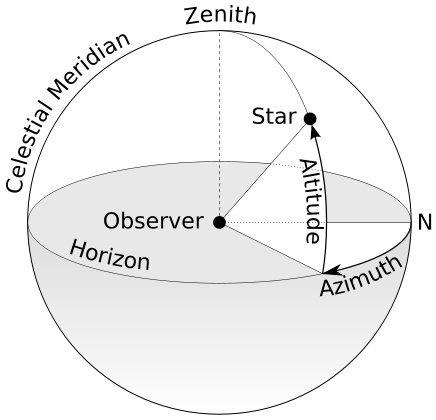
\includegraphics[width=7cm]{Azimuth-Altitude.jpg}
\end{center}
\caption{Altitude and azimuth in the horizontal coordinate system.
Source: \href{https://en.wikipedia.org/wiki/Horizontal_coordinate_system}{Wikipedia}}
\label{fig:horizontal}
\end{figure}

As shown in Figure~\ref{fig:horizontal}, the {\em altitude} and {\em azimuth} 
are defined as angles relating the direction of the star to the horizon and 
the north direction.

If the topocentric equatorial ``of date'' coordinates of an object $(X',Y',Z')$ 
are known, the altitude and azimuth can be computed as follows. First, compute the 
topocentric right ascension $\alpha$ and declination $\delta$ by 
$\alpha = {\rm arg}(X' + i Y')$ and $\delta = \sin^{-1}(Z'/R')$, where 
$R'=\sqrt{X'^2+Y'^2+Z'^2}$.
Next, calculate the hour angle, $H$, by $H=t_s-\alpha$. Here $t_s$ 
is the local apparent sidereal time LAST. 
Finally, $a$ and $A$ are related to $H$ and $\delta$ by 
\beqn
  \cos a \sin A &=& -\cos \delta \sin H \label{eq:aAFromHdel1} \\
  \cos a \cos A &=& \sin \delta \cos \phi - \cos \delta \cos H \sin \phi 
\label{eq:aAFromHdel2} \\
  \sin a &=& \sin \delta \sin \phi + \cos \delta \cos H \cos \phi .
\label{eq:aAFromHdel3}
\eeqn
The altitude computed by these formulae does not include atmospheric refraction, 
which is significant especially for objects close to the horizon.

\section{Atmospheric Refraction}

Atmospheric refraction changes the altitude of an object. The effect is particularly 
significant for objects close to the horizon. At the horizon, refraction 
can raise the altitude of an object by $34'$. Atmospheric refraction 
depends on the local temperature, pressure, humidity and other conditions. 
Sophisticated atmospheric refraction models involve numerical integration, 
but the accuracy depends on the local conditions.
On our local star chart webpage, we use a low-precision fitting formula 
to model the atmospheric refraction. 
\href{https://en.wikipedia.org/wiki/Atmospheric_refraction#cite_note-Saemundsson1986-24}{S{\ae}mundsson's formula} 
is used in which the change in altitude $\Delta a$ is given by 
\beq
  \Delta a = 1.02' \left(\frac{P}{101~{\rm kPa}}\right) 
\left( \frac{283~{\rm K}}{T}\right)  
\cot \left(a + \frac{10.3^\circ}{a + 5.11^\circ}\right) ,
\label{eq:atmRefraction}
\eeq
where $T$ is temperature and $P$ is pressure. In all of our calculations, 
we use $T=286$~K and $P=101~{\rm kPa}$.

\section{Map Projections}
\label{sec:maps}

Given the positions of celestial objects in spherical coordinates (altitude, 
azimuth or GCRS Ra and Dec), the final step is to plot them on the computer 
screen, which is a two-dimensional flat surface. There are various methods 
to map a spherical surface to a flat surface. Distortion is unavoidable. 
Two projection methods are used in our star charts. 
\href{https://en.wikipedia.org/wiki/Stereographic_projection}{Stereographic projection} 
is used to generate the local star charts and the polar GCRS charts. 
\href{https://en.wikipedia.org/wiki/Mollweide_projection}{Mollweide projection} 
is used to generate the all-sky GCRS chart. 

Stereographic projection is commonly used in sky maps. The mapping is 
conformal and shapes are preserved over a small area. However, 
the mapping does not preserve area. For example, in the local star charts 
a constellation is about twice as big when it is near the horizon than 
when it is near the zenith. This effect is quite noticeable in animations 
showing the diurnal motion of the sky. This feature might not be as bad, 
since constellations do appear bigger when they are close to the horizon 
because of the \href{https://www.skyandtelescope.com/observing/moon-illusion-confusion11252015/}{Moon illusion}. 
However, it should be noted that stereographic projection is not 
designed to model the Moon illusion.

Mollweide projection preserves areas but not angles. There is significant 
distortion in shapes in regions far away from the equator.

\subsection{Local Star Charts}

The \href{../sidereal.html}{local star charts} are based on the horizontal 
coordinate system. The coordinates are $(a,A)$ (altitude and azimuth). The mapping 
from $(a,A)$ to the 2D flat surface $(x_g,y_g)$ is done by the stereographic projection 
with the nadir as the projection point. 
Only objects above or on the horizon ($a \geq 0$) are plotted.

\begin{figure}[h]
\begin{center}
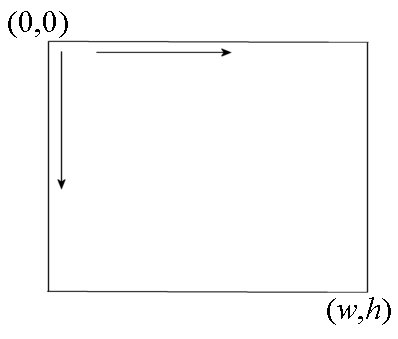
\includegraphics[width=6cm]{computerGraphics.jpg}
\end{center}
\caption{Graph coordinates in canvas. The origin is at the upper-left corner. 
The $x$ coordinate increases to the right and $y$ coordinates increases downward. 
The coordinate of the lower-right corner is $(w,h)$, where $w$ is the width 
and $h$ is the height of the canvas.}
\label{fig:computerGraphics}
\end{figure}

Before describing the equation of the mapping, it is useful to understand how the 
graph coordinate system is oriented. Graphs are drawn using the HTML canvas. 
As shown in Figure~\ref{fig:computerGraphics}, in the HTML canvas coordinates $(x_g,y_g)$
the upper-left corner is the origin $(x_g,y_g)=(0,0)$. The $x$ coordinate increases to the 
right and $y$ coordinates increases downward. The coordinate of the lower-right 
corner is $(x_g,y_g)=(w,h)$, where $w$ is the width and $h$ is the height of the canvas 
in pixels. In the local star charts, we set $w=h=800$~pixels.

The mapping $(a,A) \rightarrow (x_g,y_g)$ is given by 
\beq 
  r = r_h \tan\left( \frac{\pi}{4} -\frac{a}{2}\right) \ \ , \ \ 
  x_g = \frac{w}{2} + r \sin A \ \ , \ \ y_g = \frac{h}{2} + r \cos A , 
\label{eq:stereographicHor}
\eeq
where $r_h = 0.47\max(w,h)$. The equation can be considered as two transformations: 
$a \rightarrow r$ and $(r,A) \rightarrow (x_g, y_g)$. Under this mapping, the zenith 
is mapped to the center of the canvas. Contours of $a$ are circles 
of radius $\tan(\pi/4 - a/2)$ centered at the center of the canvas. Thus, the value of 
$r_h$ is the radius of the horizon. The value 0.47 is to make rooms for drawing labels 
outside the horizon.

\subsection{GCRS Star Charts}

\subsubsection{Polar Charts} 

The first chart is centered at the GCRS north pole. It is generated by 
the stereographic projection with the GCRS south pole as the projection 
point. Only the region in the northern hemisphere is shown. The third chart 
is centered at the GCRS south pole. It is generated by the stereographic projection 
with the GCRS north pole as the projection point. 

In general, if $\alpha_c$ and $\delta_c$ are the GCRS right ascension and declination 
at the center of the chart. The mapping $(\alpha,\delta) \rightarrow (x_g,y_g)$ is 
given by 
\beqn
  x_g &=& \frac{w}{2} + \frac{r_h (\cos \delta_c \sin \delta 
- \sin \delta_c \cos \delta \cos \Delta \alpha )}{1 + \sin \delta_c \sin \delta 
+ \cos \delta_c \cos \delta \cos \Delta \alpha} ,
\label{eq:stereographicXg} \\ \cr
  y_g &=& \frac{h}{2} - \frac{r_h \cos \delta \sin \Delta \alpha}{1 + 
\sin \delta_c \sin \delta + \cos \delta_c \cos \delta \cos \Delta \alpha} , 
\label{eq:stereographicYg}
\eeqn
where $r_h = 0.465\max(w,h)$ and $\Delta \alpha = \alpha - \alpha_c$. 
The width and height are set to $w=h=700$~pixels.
For the first chart, $\delta_c=\pi/2$. For the third chart, $\delta_c=-\pi/2$. 
The value of $\alpha_c$ determines the orientation of the GCRS Ra lines. 
For example, if $\alpha_c=0$ in the first chart, the line $\alpha=0$ 
is a horizontal line from the graph center $(w/2,h/2)$ to the 
middle left point $(w/2 - r_h, h/2)$. 

Note that when $\delta_c=\pi/2$, $\delta = a$ and $\Delta \alpha = -\pi/2 - A$, 
equations~(\ref{eq:stereographicXg}) and (\ref{eq:stereographicYg}) reduce 
to equation~(\ref{eq:stereographicHor}) since it can be shown that 
$\tan(\pi/4 - a/2) = \cos a/(1+\sin a)$.

\subsubsection{All-Sky Chart} 

The second GCRS chart is an all-sky chart. The GCRS right ascension at the center 
is set by the parameter $\alpha_c$. The canvas width and height are $w=800$~pixels 
and $h=400$~pixels. The chart is generated by the Mollweide 
projection. The mapping $(\alpha, \delta) \rightarrow (x_g,y_g)$ is given by 
\beq
  x_g = \frac{w}{2} - r_h P\left( \frac{\alpha-\alpha_c}{\pi}\right) \cos \theta 
\ \ , \ \ y_g = \frac{h}{2} - \frac{r_h}{2} \sin \theta , 
\label{eq:mollweide}
\eeq
where $r_h = 0.465\max(w,h)$ and $\theta$ satisfies the equation 
\beq
  2\theta + \sin 2\theta = \pi \sin \delta .
\eeq 
The above equation is solved by the Newton-Raphson method. The Newton-Raphson 
method usually converges to machine roundoff precision within 6 iterations. 
However, it may fail very close to the poles ($|\delta|\approx \pi/2$). 
When the Newton solver fails to converge after 20 iterations, the method 
of bisection is used instead, but this rarely, if ever, occurs.

In equation~(\ref{eq:mollweide}), the function $P$ is defined as 
\beq
  P(x) = x - 2 \cdot {\rm int}\left( \frac{x+1}{2} \right) 
\eeq
so that $P(x) \in [-1,1)$ for any $x\in (-\infty, \infty)$.
This means that $x_g \in [w/2 - r_h, w/2 + r_h)$ and all points are inside 
an ellipse centered at $(w/2,h/2)$ with a semi-major axis of $r_h$ and 
a semi-minor axis of $r_h/2$.

\subsection{Joining Two Points by a Straight Line}

In some cases (e.g.\ drawing constellation lines), we want to join 
two points $\ve{r_{g1}}=(x_{g1},y_{g1})$ 
and $\ve{r_{g2}}=(x_{g2},y_{g2})$ by a straight line on canvas. 
This is straightforward in most cases. However, 
in the stereographic charts, only half of the celestial sphere is plotted. 
If both points are inside the chart, a straight line is drawn without any 
problem. If both points are outside the chart, no line will be drawn (even 
though it is possible to have a portion of the line inside the chart). 
The problem arises if one of the points is outside the chart. In this case, 
only the part of the line inside the chart should be drawn. In the Mollweide 
chart, the whole celestial sphere is covered. However, in some cases it happens 
that the straight line connecting the two points crosses the left and right 
boundary of the chart. In this case, the line should be broken into two: one 
joining $\ve{r_{g1}}$ to the boundary and another joining $\ve{r_{g2}}$ to the 
boundary on the other side. 

In the following we describe the mathematical detail in handling these 
cases.

\subsubsection{Stereographic Charts}

A point $\ve{r_g}$ is inside the chart if $|\ve{r_g}-\ve{r_c}| \leq r_h$, 
where $\ve{r_c}=(w/2,h/2)$ is the position vector of the canvas center. 
Let $\ve{\xi}=\ve{r_g}-\ve{r_c}$. Also denote $\ve{\xi_1}=\ve{r_{g1}}-\ve{r_c}$ 
and $\ve{\xi_2}=\ve{r_{g2}}-\ve{r_c}$. Suppose that one of the two points is 
outside the chart. Then we have either $|\ve{\xi_1}|>r_h$ or $|\ve{\xi_2}|>r_h$. 
We will then replace the point outside the chart by a point on the line and on 
the chart boundary. Points on the straight line joining $\ve{r_{g1}}$ and 
$\ve{r_{g2}}$ can be described by the parametric equation 
\beq
  \ve{\xi}(s) = \ve{\xi_1} + s(\ve{\xi_2}-\ve{\xi_1}) ,
\eeq
where $s \in [0,1]$. We want to find $s$ so that $|\ve{\xi}(s)|=r_h$, 
which is a quadratic equation in $s$. The solution of the quadratic equation 
is given by 
\beq
  s_{\pm} = \frac{\xi_1^2 - \ve{\xi_1}\cdot \ve{\xi_2} \pm 
\sqrt{(\xi_1^2 - \ve{\xi_1}\cdot \ve{\xi_2})^2 + (r_h^2-\xi_1^2) |\ve{\xi_2}-\ve{\xi_1}|^2}}
{|\ve{\xi_2}-\ve{\xi_1}|^2} .
\eeq
The solution $s=s_+$ should be used if $|\ve{\xi_2}|>r_h$ and $s=s_-$ should be 
used if $|\ve{\xi_1}|>r_h$.

In summary, if $\ve{r_{g2}}$ is outside the chart, the straight line should be 
the line joining $\ve{r_{g1}}$ to $\ve{r_{g3}}$, where 
\beq
  \ve{r_{g3}} = \ve{r_{g1}} + s_+ (\ve{r_{g2}}-\ve{r_{g1}}) .
\eeq
If $\ve{r_{g1}}$ is outside the chart, the straight line should be
the line joining $\ve{r_{g2}}$ to $\ve{r_{g3}}$, where
\beq
  \ve{r_{g3}} = \ve{r_{g1}} + s_- (\ve{r_{g2}}-\ve{r_{g1}}) .
\eeq

\subsubsection{Mollweide Chart} 

The central GCRS Ra is specified by the parameter $\alpha_c$. The left and 
right boundary of the chart is $\alpha=\alpha_c +\pi$. Given two points 
$\ve{r_{g1}}$ and $\ve{r_{g2}}$, we need to determine whether the line 
joining them crosses the boundary. First, calculate the following three quantities
\beq
  \Delta x_1 = P \left(\frac{\alpha_1-\alpha_c-\pi}{\pi}\right) \ \ , \ \ 
  \Delta x_2 = P\left(\frac{\alpha_2-\alpha_c-\pi}{\pi}\right) \ \ , \ \
  \Delta x_{12} = P\left(\frac{\alpha_1-\alpha_2}{\pi}\right) .
\eeq
The line will cross the 
boundary if the following conditions are satisfied: (1) $\Delta x_1 \Delta x_2 <0$ 
and (2) $|\Delta x_1| + |\Delta x_2| = |\Delta x_{12}|$. The first 
condition says that $\alpha_1$ and $\alpha_2$ are on the opposite side of the 
boundary Ra. The second condition says that the line that crosses the Ra boundary is 
the shortest line joining the two points. As an example, suppose 
$\ve{r_{g1}}=(-\pi/4,\delta_1)$, $\ve{r_{g2}}=(\pi/2,\delta_2)$ and 
$\alpha_c=0$. It follows that $\Delta x_1 = 3/4$, $\Delta x_2=-1/2$ and 
$\Delta x_{12}=-3/4$. It is clear that $\alpha_1$ and $\alpha_2$ are on 
opposite sides of the boundary Ra $\alpha_b=\pi$, but the shortest line 
joining the two point passes through $\alpha=0$ instead of $\alpha=\pi$ 
and so the line does not cross the boundary Ra. The second condition is 
violated in this case. Suppose that $\alpha_c=\pi$. Then the boundary Ra 
is $\alpha_b=0$ and so the line crosses the boundary. In this case, 
$\Delta x_1=-1/4$, $\Delta x_2=1/2$, $\Delta x_{12}=-3/4$, and both 
conditions are indeed satisfied.

Suppose that the shortest line joining the two points does cross the 
boundary Ra. We need to split the line into two: a line joining 
$\ve{r_{g1}}$ and $\ve{r_{g3}}$, and a line joining $\ve{r_{g2}}$ and 
$\ve{r_{g4}}$, where $\ve{r_{g3}}$ is on the chart boundary closest 
to $\ve{r_{g1}}$ and $\ve{r_{g4}}$ is on the chart boundary closest to 
$\ve{r_{g2}}$.

To calculate $\ve{r_{g3}}$, first compute the following vectors 
\beq
  \ve{\xi_1} = \frac{\ve{r_{g1}}-\ve{r_c}}{r_h} \ \ , \ \ 
  \ve{\xi_2} = \frac{\ve{r_{g2}}-\ve{r_c}}{r_h} .
\eeq
Next compute $\ve{\xi'_2} = (\xi'_{2x} , \xi_{2y})$, where 
\beq
  \xi'_{2x} = \left \{ \begin{array}{ll} \xi_{2x} + 2\cos \theta_2 & {\rm if }~x_1>0 \\ 
\xi_{2x} -2\cos \theta_2 & {\rm if }~x_1 < 0 \end{array} \right. ,
\eeq
and $\theta_2$ satisfies the equation $2\theta_2 + \sin 2\theta_2 = \pi \sin \delta_2$. 
Defined in this way, the point $\ve{r'_{g2}}=\ve{x_c}+r_h \ve{\xi'_2}$ is outside the 
chart. Now we want to find $\ve{r_{g3}}$ on the line joining $\ve{r_{g1}}$ and 
$\ve{r'_{g2}}$ and on the chart boundary. Points on the line joining 
$\ve{r_{g1}}$ and $\ve{r'_{g2}}$ can be parameterized by the equation 
\beq
  \ve{\xi}(s) = \ve{\xi_1} + s(\ve{\xi'_2} - \ve{\xi_1}) , 
\eeq
where $s \in [0,1]$. The boundary of the chart is an ellipse centered at $\ve{r_c}$ 
with a semi-major axis $r_h$ and a semi-minor axis $r_h/2$. Hence, 
the point $\ve{\xi}$ is on the boundary if $\xi_x^2 + 4\xi_y^2=1$, which is a quadratic 
equation in $s$. The solution is given by 
\beqn
  s &=& \frac{1-\xi_{1x}^2 - 4\xi_{1y}^2}{\xi_{1x}\Delta \xi_x + 4\xi_{1y} \Delta \xi_y 
+ \sqrt{(\xi_{1x}\Delta \xi_x + 4\xi_{1y}\Delta \xi_y)^2 + 
(\Delta \xi_x^2 + 4\Delta \xi_y^2)(1-\xi_{1x}^2 - 4\xi_{1y}^2)}} , \cr \cr 
 \Delta \xi_x &=& \xi'_{2x}-\xi_{1x} \ \ , \ \ 
 \Delta \xi_y = \xi_{2y} - \xi_{1y} ,
\eeqn
and $\ve{r_{g3}}$ is given by 
\beq
  \ve{r_{g3}} = \ve{r_c} + r_h[\ve{\xi_1} + s(\ve{\xi'_2}-\ve{\xi_1})] 
 = \ve{r_{g1}} + r_h s (\ve{\xi'_2}-\ve{\xi_1}) .
\eeq
Having computed $\ve{r_{g3}}=(x_{g3},y_{g3})$, $\ve{r_{g4}}=(x_{g4},y_{g4})$ 
can be computed by the equation 
\beq
  x_{g4} = \frac{w}{2}-x_{g3} \ \ , \ \ y_{g4} = y_{g3} .
\eeq

\section{Plotting Equator, Ecliptic and Galactic Equator} 

Ecliptic is plotted on a local star chart when the Ecliptic button below 
the chart is active. Ecliptic is plotted on the GCRS charts when the 
Ecliptic button on the GCRS page is active. Galactic equator, as well as 
Milky Way boundary, is plotted 
on a local star chart when the Milky Way button below the chart is active. 
Galactic equator, as well as Milky Way boundary, is plotted on the GCRS 
charts when the Milky Way button on the GCRS page is active. 

In this section, we discuss the mathematical detail in plotting the 
equator, ecliptic and galactic equator, which are all great circles on 
the celestial sphere. They can be defined as the plane perpendicular to 
a pole. The general strategy is first to calculate the position of the pole 
in the coordinate system the chart is based on. Then the coordinates of points 
on the great circle perpendicular to the pole can be parameterized by a parameter 
$\theta$.

\subsection{Local Star Charts} 

The coordinate system the local star charts based on is the horizontal 
coordinate system. We first calculate the altitude $a_p$ and azimuth $A_p$ 
of the pole. Either a north pole or a south pole will work. We choose the 
north pole. 

The ``of date'' declination of the celestial north pole is $\delta=\pi/2$. 
The ``of date'' Ra and Dec of the ecliptic north pole are $\alpha_p=-\pi/2$ and 
$\delta_p = \pi/2-\epsilon_A$, where the obliquity of the ecliptic of date 
is computed by equation~(10) and Table~3 in
\href{http://adsabs.harvard.edu/abs/2011A%26A...534A..22V}{Vond\'rak,
Capitaine and Wallace}. 
The Ra and Dec of the galactic north pole with respect to J2000.0 mean equator 
and equinox are $\alpha_{p0} = 12^{\rm h} 51^{\rm m} 26^{\rm s}$ and 
$\delta_{p0} = 27^\circ 07' 42''$. The ``of date'' mean equatorial coordinates 
at other times are computed
by applying the precession matrix on the J2000.0 coordinates. Specifically, 
the vector $\ve{X_p}=\ve{P_0}(T) \ve{X_{p0}}$ is calculated, where $\ve{X_{p0}}$ is 
a column vector defined as 
\beq
  \ve{X_{p0}}=(\cos \alpha_{p0} \cos \delta_{p0}\ \sin \alpha_{p0} \cos \delta_{p0} \ 
\sin \delta_{p0})^T
\eeq
and the precession matrix $\ve{P_0}(T)$ is calculated by 
equations~(20), (11), (13), Tables~4, 6 in 
\href{http://adsabs.harvard.edu/abs/2011A%26A...534A..22V}{Vond\'rak, Capitaine and Wallace}. 
The ``of date'' Ra and Dec of the galactic north pole is then given by 
$\alpha_p = {\rm arg}(X_p+iY_p)$ and $\delta_p = \sin^{-1} Z_p$. 
Note that $|\ve{X_p}|=|\ve{X_{p0}}|=1$ by construction.

Having computed the ``of date'' mean equatorial position of the pole, the hour angle 
is calculated approximately by $H_p=t_s - \alpha_p$, where $t_s$ is the local mean 
sidereal time (LMST) computed by $t_s = {\rm GMST}+\lambda$. 
Here $\lambda$ is the longitude of the location and GMST is computed
by equation~(\ref{eq:GMST}). Note that we do not
use LAST and the apparent position in the computation because the correction is
small and can be ignored for plotting purpose.

The altitude $a_p$ and azimuth $A_p$ are obtained by 
equations~(\ref{eq:aAFromHdel1})--(\ref{eq:aAFromHdel3}). Next calculate a vector 
$\ve{r_p} = (\cos A_p \cos a_p, \sin A_p \cos a_p, \sin a_p)$, which is a unit 
vector pointing in the direction of the pole in the horizontal coordinate system.
Denote $\ve{r_z}=(0,0,1)$ the unit vector pointing towards the zenith. Define two 
unit vectors $\ve{V}$ and $\ve{W}$ as follows:
\beq
  \ve{V} = \frac{\ve{r_z}\times \ve{r_p}}{|\ve{r_z}\times \ve{r_p}|} \ \ , \ \ 
  \ve{W} = \ve{r_p} \times \ve{V} .
\eeq
It follows that both $\ve{V}$ and $\ve{W}$ are perpendicular to $\ve{r_p}$ and so 
are on the great circle we want to plot. The great circle can be parameterized by 
the unit vector
\beq
  \ve{C}(\theta) = \cos \theta \, \ve{V} + \sin \theta \, \ve{W} ,
\eeq
where $\theta \in [0,2\pi)$. The altitude and azimuth associated with 
$\ve{C}(\theta)$ are $A(\theta)={\rm arg}(C_x(\theta) + i C_y(\theta))$ and 
$a(\theta) = \sin^{-1} C_z(\theta)$. The set of points $\{ a(\theta), A(\theta) \}$, 
$\theta \in [0,2\pi)$ represents the great cicle in the horizontal coordinate 
system. In addition, it is easy to show that 
\beq
  \ve{r_z} \cdot \ve{C}(\theta) = \frac{1-(\ve{r_z}\cdot \ve{r_p})^2}
{|\ve{r_z}\times \ve{r_p}|} 
\sin \theta .
\eeq
It follows that $\ve{r_z} \cdot \ve{C}(\theta) \geq 0$ for $\theta \in [0,\pi]$. 
These are the points on the great circle that are above or on the horizon. 
The canvas coordinates of these points are calculated by 
equation~(\ref{eq:stereographicHor}). These points can then be joined by a 
curve representing the great circle on the canvas.

\subsection{GCRS Charts} 

The coordinate system is the GCRS equatorial coordinate system, which is essentially 
the same as the J2000.0 mean equatorial coordinate system except for the 
23-milliarcsecond offset between their poles. We treat these two systems 
as identical because of the small offset. In this coordinate system, the 
coordinates of the north pole of the ecliptic of date are $\alpha_p = \gamma-\pi/2$ 
and $\delta_p = \pi/2 - \varphi$. The angles $\gamma$ and $\varphi$ are 
calculated from equation~(14) and Table~7 in
\href{http://adsabs.harvard.edu/abs/2011A%26A...534A..22V}{Vond\'rak,
Capitaine and Wallace}. The coordinates of the galactic north pole are 
$\alpha_{p} = 12^{\rm h} 51^{\rm m} 26^{\rm s}$ and $\delta_{p} = 27^\circ 07' 42''$. 

The procedure of plotting the great circle perpendicular to the pole is similar 
to that described in the previous subsection. 
The unit vector associated with the pole is computed by 
$\ve{r_p} = (\cos \alpha_p \cos \delta_p, \sin \alpha_p \cos \delta_p, \sin \delta_p)$. 
The unit vector associated with the GCRS north pole is $\ve{r_z}=(0,0,1)$. 
Define two unit vectors 
\beq
  \ve{V} = \frac{\ve{r_z}\times \ve{r_p}}{|\ve{r_z}\times \ve{r_p}|} \ \ , \ \
  \ve{W} = \ve{r_p} \times \ve{V} .
\eeq
It follows that both $\ve{V}$ and $\ve{W}$ are perpendicular to $\ve{r_p}$ and so 
are on the great circle we want to plot. The great circle can now be parameterized 
by the unit vector 
\beq
  \ve{C}(\theta) = \cos \theta \, \ve{V} + \sin \theta \, \ve{W} ,
\eeq
where $\theta \in [0,2\pi)$. The GCRS Ra and Dec associated with $\ve{C}(\theta)$ are 
$\alpha(\theta) = {\rm arg}(C_x(\theta) + i C_y(\theta))$ and 
$\delta(\theta) = \sin^{-1} C_z(\theta)$. The set of points 
$\{ \alpha(\theta), \delta(\theta) \}$,
$\theta \in [0,2\pi)$ represents the great cicle in the GCRS coordinate
system. The canvas coordinates of these points are given by 
equations~(\ref{eq:stereographicXg})--(\ref{eq:stereographicYg}) for the polar charts and 
equation~(\ref{eq:mollweide}) for the all-sky chart. 
Half of the great circle will appear 
on each of the polar charts and the full great circle will appear  
in the all-sky chart. 

\section{Stars}

\subsection{Database}

The star data used on our webpages are a subset of the \href{http://astronexus.com/node/34}
{HYG 3.0 database}. The database is constructed using the following procedure. 
All data processing was done using the \href{https://www.r-project.org/}{R software}.

\begin{enumerate}
\item Remove the Sun, Capella~B and $\alpha$~Cen~B from the database. 
Capella~B and Capella~A are too close to be separated on our star charts. 
They have slightly different 3D motions (constructed from the database) that 
will separate them in the distant future and distant past. That is why Capella~B 
is removed. $\alpha$~Cen~B is removed for the same reason. 

\item The ICRS rectangular coordinates of each star are computed from their 
distance $D_0$, J2000.0 $\alpha_0$ and $\delta_0$ by 
$x_0=D_0 \cos \alpha_0 \cos \delta_0$, $y_0=D_0\sin \alpha_0 \cos \delta_0$ and 
$z_0=D_0 \sin \delta_0$. These are components of the ICRS position vector 
$\ve{r(t)}$ at $t=$J2000.0. 
Note that a value of 100,000 is assigned to $D_0$ if the distance of 
a star is unknown or its value is dubious. This will not cause 
much trouble since it is the angular direction of the star we 
are interested in, but it needs to be kept in mind for calculations 
involving $D_0$.

\item ICRS components of a star's 3D velocity is computed 
from its distance $D_0$, J2000.0 $\alpha_0$ and $\delta_0$, proper 
motions $\mu_{\alpha}$, $\mu_{\delta}$ and radial velocity $v_r$ according 
to the equation 
\beqn
  \ve{v} &=& D_0 \mu_{\alpha} \ve{e_{\alpha}} + D_0\mu_{\delta} \ve{e_{\delta}}  
+ v_r \ve{e_r} , \\ 
  \ve{e_{\alpha}} &=& -\sin \alpha_0 \cos \delta_0 \ve{\hat{x}} + \cos \alpha_0 \cos \delta_0\ve{\hat{y}} \\ 
  \ve{e_{\delta}} &=& -\cos \alpha_0 \sin \delta_0 \ve{\hat{x}} 
-\sin \alpha_0 \sin \delta_0 \ve{\hat{y}} + \cos \delta_0 \ve{\hat{z}} \\ 
  \ve{e_r} &=& \cos \alpha_0 \cos \delta_0 \ve{\hat{x}} 
+ \sin \alpha_0 \cos \delta_0 \ve{\hat{y}} + \sin \delta_0 \ve{\hat{z}} .
\eeqn
All components of $\ve{v}$, $v_x$, $v_y$ and $v_z$, are converted 
to pc/(Julian century) for convenience of later calculations.

\item Our webpages draw star charts in the time range J2000.0$\pm$200,000 years. 
For stars with reliable measured distance ($D_0 \neq 10^5$), their minimum 
distance and magnitude in the time intervals J2000.0$\pm$200,000 years are 
calculated as follows. The ICRS position vector of the star as a function of $t$ 
(neglecting light-time correction) is given by 
\beq
  \ve{r}(t) = \ve{r_0} + \ve{v} \Delta t ,
\eeq
where $\ve{r_0}$ is the position vector of the star at $t=t_0$=J2000.0 and 
$\Delta t = t-t_0$. Here we assume that the star moves with a constant 
velocity $\ve{v}$. The distance is minimum when $\ve{v}\cdot \ve{r}(t)=0$, 
which gives 
\beq
  \Delta t_{\rm min} = -\frac{\ve{r_0}\cdot \ve{v}}{v^2} .
\eeq
Since we are only interested in $|\Delta t|<2\times 10^5$~years, we set 
$\Delta t_{\rm min} =-2\times 10^5$~years if $\Delta t_{\rm min}< -2\times 10^5$~years  
and $\Delta t_{\rm min} =2\times 10^5$~years if $\Delta t_{\rm min}> 2\times 10^5$~years. 
Then the minimum distance in the time interval is 
\beq
  D_{\rm min} = |\ve{r_0} + \ve{v} \Delta t_{\rm min}| 
\eeq
and the minimum magnitude of the star is calculated by the inverse square law as 
\beq
  m_{\rm min} = m_0 + 5 \log_{10} (D_{\rm min}/D_0) , 
\eeq
where $m_0$ is the star's magnitude at $t=t_0$ and $D_0=|\ve{r_0}|$ is 
the star's distance at $t=t_0$.

\item Stars with $m_{\rm min} > 5.3$ are removed from the database 
since 5.3 is the limiting magnitude of stars that will be plotted on 
our star charts. The resulting database contains 2559 stars.

\item For the purpose of drawing constellation lines, certain stars 
are manually selected for each constellation line segment. They 
are specified by either the star's proper name, Bayer/Flamsteed name, 
or hip number. They are then converted to the index numbers in the database. 

\item For each of the 88 constellations, approximate values of the ICRS 
Ra and Dec of the constellation are entered manually. The constellation labels, 
when active, will be plotted at these locations. For the constellations Hydra, 
Serpens and Eridanus, two locations are indicated because of their large size 
or topology.

\item The final data are put into JSON format and outputted 
to the JavaScript file {\tt brghtStars.js}, which contains functions returning 
JavaScript objects.
\end{enumerate}

\subsection{Light-time Correction}

\href{https://en.wikipedia.org/wiki/Light-time_correction}{Light-time correction} 
arises from the finite speed of light. It is usually included in the calculation of 
the apparent positions of planets, but usually not applied to the positions of stars 
because their motion and distance are not known accurately. Our webpages 
do not include light-time correction for stars. The detail calculation is presented here 
so that it can be implemented when accurate data are available in the future. 
The equations derived in this subsection are essentially the same as those 
in \href{http://adsabs.harvard.edu/abs/1985A%26A...144..232S}{Stumpff 
[A\&A 144, 232 (1985)]}, but are derived using a different approach.

The observed barycentric position of a star at time $t$ is the ``true'' position 
of the star at the retarded time $t_r$ 
\beq
  \ve{r^*}(t) = \ve{r}(t_r) .
\label{def:rstar}
\eeq
The retarded time $t_r$ satisfies the equation 
\beq
  t_r(t) = t - \frac{D(t_r)}{c} ,
\label{eq:tr}
\eeq
where $D(t_r) = |\ve{r}(t_r)|$ is the barycentric distance of the star 
at the retarded time and $c$ is the speed of light. Differentiating 
equation~(\ref{def:rstar}) with respect 
to $t$ gives 
\beq
  \ve{v^*}(t) = \ve{\dot{r}^*}(t) = \ve{v}(t_r) \frac{d t_r}{dt} .
\label{eq:vstar1}
\eeq
It follows from~(\ref{eq:tr}) that 
\beq
  \frac{dt_t}{dt} = 1-\frac{v_r}{c} \frac{dt_r}{dt} \ \ \ \Rightarrow \ \ \ 
  \frac{dt_r}{dt} = \frac{1}{1+\beta_r(t_r)} ,
\label{eq:dtr_dt}
\eeq
where $v_r = d D/dt$ is the radial velocity and $\beta_r = v_r/c$. Combining 
equations~(\ref{eq:vstar1}) and (\ref{eq:dtr_dt}) gives 
\beq
  \ve{v^*}(t) = \frac{\ve{v}(t_r)}{1+\beta_r(t_r)} .
\eeq
Thus, the observed tangential velocity, $\ve{v^*}_T(t)=D\mu_{\alpha}\ve{e_{\alpha}} 
+ D \mu_{\delta} \ve{e_{\delta}}$ is related to the true 
tangential velocoty at the retarded time $\ve{v}_T(t_r)$ by 
\beq
   \ve{v^*}_T(t) = \frac{\ve{v}_T(t_r)}{1+\beta_r(t_r)} .
\label{eq:vTstar}
\eeq
This formula explains the origin of the observed 
\href{https://en.wikipedia.org/wiki/Superluminal_motion}{superluminal motion} 
of jets in some active galaxies: if a jet moving close to the speed of light 
is moving at a very small angle towards the observer, $1+\beta_r \ll 1$ and 
it is possible to have $v^*_T > c$. Equation~(\ref{eq:vTstar}) is usually derived by 
drawing a figure showing the geometry between the source and observer. 
The derivation presented here is mathematically more straightforward but 
the physics behind the formula is illustrated more clearly in the conventional 
derivation. For stars in the vicinity of the Sun, 
$\beta_r \sim 10^{-4}$ and so the correction to the tangential 
velocity is very small. The radial velocity $v_r$ is related to the redshift $z$ 
by the special relativistic Doppler formula 
\beq
  1 + z = \frac{1+\beta_r}{\sqrt{1-\beta^2}} ,
\label{eq:z}
\eeq
where $\beta = v/c = \sqrt{v_T^2+v_r^2}/c$. Thus, equations~(\ref{eq:vTstar}) 
and (\ref{eq:z}) must be solved together to obtain $\ve{v}_T$ and $v_r$ 
from the observed quantities $\ve{v^*}_T$ and $z$. Once $\ve{v}_T$ and 
$v_r$ are computed, the true velocity $\ve{v}(t_r)$ is obtained. We will assume that 
$\ve{v}$ is constant, which is in general a good approximation since the time scale of 
galactic rotation in the solar neighborhood is $10^8$ years and we are considering 
a much shorter time span.

Suppose the apparent position at time $t_0$, $\ve{r^*}(t_0)$, and the 
velocity $\ve{v}$ is known, the observed position at time $t=t_0+\Delta t$ 
is given by 
\beq
  \ve{r^*}(t) = \ve{r}(t_r(t))  
\label{eq:rstar1}
\eeq
with 
\beqn
  t_r(t) &=& t - \frac{D(t_r(t))}{c} = t_0 + \Delta t - \frac{D(t_r(t_0))}{c} 
+ \frac{D(t_r(t_0)) - D(t_r(t))}{c} \cr \cr
&=& t_r(t_0) + (1+f) \Delta t ,
\label{eq:tr2}
\eeqn
where 
\beq
  f = \frac{D(t_r(t_0))-D(t_r(t))}{c \Delta t} .
\label{eq:f1}
\eeq
Denote $\ve{r^*_0} = \ve{r^*}(t_0) = \ve{r}(t_r(t_0))$, 
$D_0 = D(t_r(t_0)) = |\ve{r^*_0}|$, 
and $D=D(t_r(t))=|\ve{r^*}(t)|$. It follows from equation~(\ref{eq:rstar1}), 
(\ref{eq:tr2}) and $\ve{r}(t_2) = \ve{r}(t_1) + \ve{v}(t_2-t_1)$ that 
\beq
  \ve{r^*}(t) = \ve{r^*_0} + (1+f)\ve{v} \Delta t .
\label{eq:rstar2}
\eeq
It follows from~(\ref{eq:f1}) that 
\beq
  D = D(t_r(t)) = |\ve{r^*}(t)| = D_0 - f c \Delta t .
\label{eq:D}
\eeq
Combining equations~(\ref{eq:rstar2}) and (\ref{eq:D}) yields 
\beq
  D_0 - f c \Delta t = |\ve{r^*_0} + (1+f)\ve{v} \Delta t| .
\eeq
Squaring both sides of the above equation gives 
\beq
  (D_0 - f c \Delta t)^2 = D_0^2 + 2(1+f)\Delta t \ve{r^*_0} \cdot \ve{v} 
+ (1+f)^2 v^2 \Delta t^2 .
\eeq
This is a quadratic equation in $f$ and the solution is given by 
\beq
  f = -\frac{2 \ve{s_0}\cdot \ve{\beta} + \beta^2 \Delta t}{s_0 + 
\ve{s_0}\cdot \ve{\beta} + \beta^2 \Delta t + \sqrt{Q}} ,
\label{eq:f2}
\eeq
where $\ve{s_0} = \ve{r^*_0}/c$, $\ve{\beta}=\ve{v}/c$, $s_0 = |\ve{s_0}|$, 
$\beta = |\ve{\beta}|$ and 
\beq
  Q = (s_0 + \ve{s_0}\cdot \ve{\beta} + \beta^2 \Delta t)^2 + 
(1-\beta^2)(2\ve{s_0}\cdot \ve{\beta} + \beta^2 \Delta t) .
\eeq
Equations~(\ref{eq:rstar2}) and (\ref{eq:f2}) can be used to update the 
apparent position of a star from time $t_0$ to $t$. The term $f\ve{v}\Delta t$ 
is an extra term arising from the light-time correction. The value of $f$ is 
of order $\beta$, which is $\sim 10^{-4}$ for stars in the solar neighborhood. 
Since the fractional accuracy of $\ve{v}$ is much larger than $10^{-4}$ in the 
data used by our webpages, including the light-time correction will not 
improve the accuracy of a star's position.

\subsection{Plotting Stars} 
\label{sec:plottingStars}

Geocentric apparent positions of stars at a given time are required to plot 
the stars in the GCRS star charts. Topocentric apparent positions of stars 
are required to plot the stars in the local star charts. 
Chapter~7 of \expl provides a detailed procedure in computing the apparent 
positions of stars. For geocentric apparent positions, the stars' 
space motion, \href{https://en.wikipedia.org/wiki/Parallax}{annual parallax}, 
\href{http://www.einstein-online.info/spotlights/light_deflection.html}{gravitational 
deflection of light} by the Sun, and \href{https://en.wikipedia.org/wiki/Aberration_of_light}
{annual aberration of light} should be included. 
For topocentric positions, precession, nutation, polar motion, 
\href{https://en.wikipedia.org/wiki/Aberration_of_light}
{diurnal aberration of light} and atmospheric refraction should also be included. 

Apart from precession and space motion, all the other effects mentioned 
are periodic or nonaccumulative. Annual parallax is 
inversely proportional to the star's distance. It is very small. The parallax 
of the closest stars is about $0.75''$. Gravitational deflection of light is 
only significant if the star is in a direction very close to the Sun. However, 
the maximum deflection angle is only $1.75''$. Annual aberration of light causes a shift 
in a star's position by $20.5''$ over the course of a year. The effect of 
nutation is about $9''$. The effect of diurnal aberration is smaller than $0.32''$. Polar 
motion affects a star's position by about $0.3''$. Atmospheric refraction 
can change a star's position by $34'$ if it is close to the horizon. 
On our webpages, we only include the space motion, precession and atmospheric 
refraction for plotting stars.

A star's ICRS position at time $t$ (neglecting light-time correction) 
is calculated according to the equation 
\beq
  \ve{r}(t) = \ve{r_0} + \ve{v} (t-t_0) ,
\eeq
where $t_0=$J2000.0 and $\ve{r_0} = D_0 (\cos \alpha_0 \cos \delta_0\ 
\sin \alpha_0 \cos \delta_0\ \sin \delta_0)^T$ is the ICRS position 
vector at $t=t_0$, $\alpha_0$ and $\beta_0$ are the star's ICRS Ra and Dec 
at J2000.0, and $D_0=|\ve{r_0}|=\sqrt{\ve{r_0}^T \ve{r_0}}$ is the distance 
of the star at $t=t_0$. Since parallax is ignored, the star's GCRS position 
is the same as its ICRS position: $\ve{X}(t)=\ve{r}(t)$. The GCRS Ra and Dec 
of the star at time $t$ is therefore $\alpha = {\rm arg}(X+iY)$ and 
$\delta = \sin^{-1} (Z/D)$, where $D=|\ve{X}(t)|=|\ve{r}(t)|$. The 
magnitude of the star at time $t$ is 
\beq
  m(t) = m_0 + 5\log_{10}(D/D_0) ,
\eeq
where $m_0$ is the star's magnitude at $t=t_0$. The star can now be 
plotted on the GCRS star charts: its canvas coordinates on the 
star charts are given by equations~(\ref{eq:stereographicXg})--(\ref{eq:mollweide}).  
A star is represented by a filled circle with size proportional to its 
magnitude $m(t)$.

To plot a star on the local star charts, we need to compute its altitude $a$ 
and azimuth $A$ at the given location. First, the ``of date'' equatorial 
coordinates are computed by the precession matrix: $\ve{X'}(t)=\ve{P_0}(T)\ve{X}(t)$, 
where $T$ is the TT Julian centuries of $t$ from $t_0$. The precession matrix 
$\ve{P_0}(T)$ is calculated by equations~(20), (11), (13), Tables~4, 6 in
\href{http://adsabs.harvard.edu/abs/2011A%26A...534A..22V}{Vond\'rak, Capitaine and Wallace}.
The ``of date'' Ra and Dec 
of the star is $\alpha = {\rm arg}(X'+iY')$ and $\delta=\sin^{-1} (Z'/D)$. 
The hour angle of the star is $H=t_s-\alpha$, where $t_s$ is the local 
sidereal time (LMST) computed by $t_s = {\rm GMST}+\lambda$. 
Here $\lambda$ is the longitude of the location and GMST is computed 
by equation~(\ref{eq:GMST}). Next $a$ and $A$ are computed using 
equations~(\ref{eq:aAFromHdel1})--(\ref{eq:aAFromHdel3}). Then the altitude 
is adjusted by the atmospheric refraction according to equation~(\ref{eq:atmRefraction}). 
The star can now be plotted on a local star chart: its canvas coordinates are 
given by equation~(\ref{eq:stereographicHor}).

\subsection{Popup Box} 
\label{sec:starsPopup}

Stars in the charts can be clicked and a popup box 
will appear. The popup box shows further information about the star: its name, 
constellation, 
apparent magnitude, distance, spectral type, color index, J2000.0 Ra and Dec, 
apparent position respect to the true equator and equinox of date, altitude, 
azimuth, rise, set and upper transit times. 

If a star's proper name is available, it is displayed in the 
popup box together with its Bayer name (e.g.\ Procyon, $\alpha$~CMi). 
If both the proper name and Bayer name are not available, Flamsteed 
name is displayed (e.g.\ 50~Cas). If proper name, Bayer name and 
Flamsteed name are not available, the HIP number is displayed (e.g.\ hip~33694). 
The constellation the star is in refers to the epoch J2000.0. Some stars 
may be in a different constellation at other times because of their space motion, 
but their constellation information will not be updated.  

When the time is between 3000~BC and 3000~AD, the position of a star 
with respect to the J2000.0 mean equator and equinox are corrected for 
proper motion and annual parallax. The apparent position with respect 
to the true equator and equinox of date are corrected for precession, 
nutation, and aberration of light in addition to proper motion and 
parallax. Outside the time interval 3000~BC -- 3000~AD, only proper 
motion is included in the J2000.0 position and only precession and 
proper motion are included in the ``of date'' position. 

A star's annual parallax is calculated by computing the star's geocentric 
position $\ve{X}$ from its BCRS position $\ve{r}$ using $\ve{X}=\ve{r}-\ve{r_E}$, 
where $\ve{r_E}$ is Earth's barycentric position, computed using 
an \href{https://ssd.jpl.nasa.gov/?planet_pos}{approximate formula} provided by JPL. 

After parallax is included, components of a star's position vector in the 
rectangular equatorial coordinates of the true equator and equinox 
of date are computed using the precession and nutation matrix: 
$\ve{X'}=\ve{NPX}$. Here $\ve{P}$ is the precession matrix $\ve{P_0}(T)$ and 
$\ve{N}$ is nutation matrix calculated by equation~(\ref{eq:nutationMatrix}).

To compute the aberration of light, we have to calculate $\ve{v_E}=\ve{\dot{r}_E}$ 
first. This is done by differentiating JPL's approximate formula for $\ve{r_E}$ 
(see the next section). The resulting $\ve{v_E}$ is expressed in the ICRS rectangular 
coordinate system. It is then transformed to the rectangular equatorial coordinate system 
of the true equator and equinox of date by applying the precession and 
nutation matrix $\ve{NPv_E}$. Then the direction 
of the star is modified by the annual aberration according to equation~(\ref{eq:aberration}) 
with $\ve{n}=\ve{X'}/|\ve{X'}|$ and 
$\ve{\beta} = \ve{N P v_E}/c$. The corrected $\alpha$ and $\delta$ are given by 
$\alpha = {\rm arg}(n'_x + i n'_y)$ and $\delta = \sin^{-1} n'_z$. These are the 
apparent Ra and Dec of date displayed in the popup box of stars in the GCRS charts. 

For the popup box in the local star charts, we also include diurnal aberration of 
light by adding $\ve{NPv_E}$ to $\ve{v_{\rm spin}}$ calculated from 
equation~(\ref{eq:vspin}). The vector $\ve{n'}$ is calculated by 
equation~(\ref{eq:aberration}) with $\ve{\beta}=(\ve{NPv_E}+\ve{v_{\rm spin}})/c$. 
The resulting $\alpha$ and $\delta$ derived from $\ve{n'}$ thus include both 
annual and diurnal aberration of light. 

The computation of stellar parallax requires $\ve{r_E}$ and the computation 
of stellar aberration requires $\ve{v_E}$. Both vectors are calculated based on 
JPL's approximate formula, which is accurate only in the time interval between 
3000~BC and 3000~AD. The formulae for the nutation matrix $\ve{N}$ also 
become inaccurate far away from this interval. That is why nutation, stellar parallax 
and aberration are not computed outside this time interval even in the popup box.

In the local star charts, altitude $a$ and azimuth $A$ in the popup box are 
calculated in the exact same way as in the previous subsection if the time 
is outside the interval 3000~BC and 3000~AD. When the time is between 3000~BC 
and 3000~AD, a star's apparent Ra and Dec corrected for space motion, parallax, 
precession, nutation and aberration of light are used to compute $a$ and $A$. 
Specifically, the hour angle is computed using $H=t_s-\alpha$, where $t_s$ 
is the local apparent sidereal time calculated from 
$t_s={\rm GAST}+\lambda$. The Greenwich apparent sidereal time is calculated 
using ${\rm GAST = GMST} - E_e$, with GMST computed from equation~(\ref{eq:GMST}) 
and $E_e$ computed from equations~(\ref{eq:Ee}), (\ref{eq:Dpsi}) and (\ref{eq:epsA}). 
Next $a$ and $A$ are computed using
equations~(\ref{eq:aAFromHdel1})--(\ref{eq:aAFromHdel3}). Then the altitude
is adjusted by the atmospheric refraction according to equation~(\ref{eq:atmRefraction}).

\section{Sun and Planets}

\subsection{Approximate Positions of Planets} 

For the purpose of plotting the Sun and planets on the star charts, the
heliocentric position $\ve{r}$ of each of the eight planets in the solar system 
is computed by the \href{https://ssd.jpl.nasa.gov/?planet_pos}{low-precision formulae} 
provided by JPL (also given in Section~8.10 of \expl). The formulae are based on 
Kepler's equations of motion with the osculating orbital elements determined 
by fitting the JPL ephemerides. The approximate heliocentric 
velocity $\dot{\ve{r}}$ can be derived by differentiating the position 
vector from the approximate formulae. Time derivatives of the orbital elements 
that are unchanged in the absence of perturbation are ignored. In other words, 
the computed $\dot{\ve{r}}$ is based on Kepler's equations of motion applied 
on the osculating orbit.
The geocentric position of a planet, including the light-time correction, is calculated 
using the equation 
\beq
  \ve{X}(t) = \ve{r}(t_r) - \ve{r}_{EM}(t) 
\approx \ve{r}(t) - \dot{\ve{r}}(t) \Delta t - \ve{r}_{EM}(t) ,
\label{eq:GCRSplanets}
\eeq
where $\ve{r}_{EM}$ is the heliocentric position of the 
Earth-Moon barycenter and the light time is approximated by 
$\Delta t \approx |\ve{r}(t) - \ve{r}_{EM}(t)|/c$. 
Note that we ignore the small difference between the heliocentric position of 
the Earth-Moon barycenter and that of the Earth barycenter, which causes 
an error of order $6.5''/(D_{\rm geo}/{\rm AU})$, where $D_{\rm geo}$ is the distance of the 
planet/Sun from Earth's barycenter. This error is in general smaller than the accuracy 
of the JPL formulae. 
Equation~(\ref{eq:GCRSplanets}) is used to compute the GCRS positions 
of Mercury, Venus, Mars, Jupiter, Saturn, Uranus and Neptune. For the Sun, 
the GCRS position is simply 
\beq
  \ve{X_{\odot}}(t) = -\ve{r}_{EM}(t) .
\label{eq:GCRSsun}
\eeq
The effect of light-time correction is of order $v/c$, 
where $v$ is the orbital speed of the planet around the Sun. It follows from 
Kepler's laws that $v/c \sim 20.5''/\sqrt{a/{\rm AU}}$, where $a$ is the orbital 
semi-major axis of the planet. We see that the light-time correction is 
not very big and can be ignored for plotting purpose. It is included 
in the calculation simply because the computation of $\dot{\ve{r}}$ is 
not expensive.

The accuracy of the JPL formulae is stated on 
\href{https://ssd.jpl.nasa.gov/?planet_pos}{this page} (also given in Section~8.10 
of \expl). This accuracy is more than enough for plotting the Sun and planets 
on the star charts 
on our webpages. However, it should be noted that 
the JPL formulae are only accurate in the time interval between 3000~BC and 
3000~AD. Beyond these times, positions of the Sun and planets will be off, and 
the Sun can be seen to go off the ecliptic for times well beyond the interval.

\subsection{Plotting the Sun and Planets}

The procedure of plotting the Sun and planets is similar to that for 
stars. If high precision is required, in addition to the light-time correction,
effects including the gravitational deflection of light 
and annual aberration of light are required to compute the apparent GCRS 
positions of the planets. For topocentric positions, geocentric parallax, 
diurnal aberration of light, precession, nutation, polar motion and 
atmospheric refraction should also be included. On our webpages, we only include 
the light-time correction, precession and atmospheric refraction. The geocentric 
parallax for the Sun and planets are small enough (usually $< 10''$) to be 
neglected for plotting purpose.

Having computed the geocentric positions of the Sun and planets using 
equation~(\ref{eq:GCRSplanets}) and (\ref{eq:GCRSsun}), their GCRS Ra and 
Dec are calculated by $\alpha={\rm arg}(X+iY)$ and $\delta=\sin^{-1}(Z/D_{\rm geo})$, 
where $D_{\rm geo}=\sqrt{X^2+Y^2+Z^2}$ is the geocentric distance. The Sun 
and planets can now be plotted on the GCRS charts: their canvas coordinates on the
charts are given by equations~(\ref{eq:stereographicXg})--(\ref{eq:mollweide}). 

For the local star charts, we need to compute the altitude $a$
and azimuth $A$ at the given location. First, the ``of date'' equatorial
coordinates are computed by the precession matrix: $\ve{X'}(t)=\ve{P_0}(T)\ve{X}(t)$,
where $T$ is the TT Julian centries from J2000.0. The ``of date'' Ra and Dec
are then calculated by $\alpha = {\rm arg}(X'+iY')$ and $\delta=\sin^{-1} (Z'/D_{\rm geo})$.
The hour angle is given by $H=t_s-\alpha$, where $t_s$ is the local
sidereal time (LMST) computed by $t_s = {\rm GMST}+\lambda$.
Here $\lambda$ is the longitude of the location and GMST is computed
by equation~(\ref{eq:GMST}). Next $a$ and $A$ are computed using
equations~(\ref{eq:aAFromHdel1})--(\ref{eq:aAFromHdel3}). Then the altitude
is adjusted by the atmospheric refraction according to equation~(\ref{eq:atmRefraction}).
The Sun and planets can now be plotted on a local star chart: their canvas coordinates are
given by equation~(\ref{eq:stereographicHor}).

\subsection{Popup Box} 

The Sun and planets in the star charts can be clicked and a popup box 
will appear displaying the information: heliocentric and geocentric distance, 
angular diameter, elongation, apparent magnitude, GCRS Ra and Dec, 
topocentric Ra and Dec, altitude and azimuth, rise, set and upper transit times. 
Positions of the Sun and planets displayed in the popup box are calculated by more 
accurate formulae. The detail calculations are described below.

\subsubsection{Positions from VSOP87} 

Heliocentric positions of the solar system planets are calculated using the 
\href{http://neoprogrammics.com/vsop87/}{VSOP87 theory} [source
paper: \href{https://ui.adsabs.harvard.edu/#abs/1988A&A...202..309B/abstract}
{Bretagnon and Francou, A\&A 202, 309 (1988)}]. VSOP87 provides semi-analytic 
solutions for solar system planets. Parameters in the equations are fitted to the 
DE200 numerical integration of JPL. The precision of VSOP87 is better than $0.1''$ 
over the time span 1900--2100. For Mercury, Venus, Earth and Mars, the 
precision is better than $1''$ over 4000 years before and after 
J2000.0. For Jupiter and Saturn, the precision is better than $1''$ over 2000 years 
before and after J2000.0. For Uranus and Neptune, the precision is better than 
$1''$ over 6000 years before and after J2000.0. 

Positions of planets displayed in the popup box are calculated from 
VSOP87A, in which heliocentric positions are computed. The code 
for the heliocentric positions is obtained from the VSOP source 
code generator tool on 
\href{http://neoprogrammics.com/vsop87/source_code_generator_tool/index.php}{this webpage}. 
The Java code obtained from that page is then changed to a JavaScript code by 
replacing all the {\tt static double} by {\tt function} and then all the 
{\tt double} by {\tt var} 

To compute the geocentric position of a planet $\ve{X}(t)$, the planet's heliocentric 
position $\ve{r}(t)$ and Earth's heliocentric position $\ve{r}_E(t)$ are first computed. 
Next the light-time is estimated to be $\Delta t \approx |\ve{r}(t)-\ve{r}_E(t)|/c$. 
Then the geocentric position of the planet is calculated by $\ve{X}(t) \approx
\ve{r}(t-\Delta t) - \ve{r}_E(t)$. This acoounts for the time-light correction to the order 
$v/c$. The error is of $(v/c)^2$, which is milliarcseconds. Geocentric 
position of the Sun is simply calculated by $\ve{X_{\odot}}(t)=-\ve{r}_E(t)$. Light-time 
correction is ignored since the motion of the Sun with respect to the solar system 
barycenter is very small.

For times outside the interval 3000~BC--3000~AD, 
GCRS Ra and Dec are computed from $\ve{X}(t)$. The ``of date'' geocentric Ra and Dec are 
computed by applying the precession matrix on $\ve{X}(t)$. 
The topocentric coordinates of a planet are computed using 
equations~(\ref{eq:topoX})--(\ref{eq:topoCS}). Hence, the geocentric parallax 
is included in the topocentric Ra and Dec. The ``of date'' topocentric 
Ra and Dec are obtained by precessing the J2000.0 topocentric Ra and Dec.
Nutation, polar motion, aberration of light 
and gravitational deflection of light are not included in the computation of 
positions of the Sun and planets outside the interval 3000~BC--3000~AD. 
For times within the interval 3000~BC--3000~AD, the J2000.0 positions 
include only the light-time correction and geocentric parallax (for topocentric 
position). The apparent ``of date'' position, as well as altitude and azimuth, 
includes light-time correction, 
precession, nutation and aberration of light. The calculations are the same 
as those described in Section~\ref{sec:starsPopup}.

The apparent angular diameter $\theta$ of a planet is given by 
$\theta = D_p/D_{\rm geo}$,
where $D_p$ is the planet's diameter and $D_{\rm geo}=|\ve{X}|$ is 
its geocentric distance. Geocentric distance is sufficient for the 
angular diameter calculation even for observers on Earth's surface because 
the fractional error is of order $10^{-5}$.

\subsubsection{Elongation, Phase Angle and Fraction of Planet Illuminated}

\begin{figure}[h]
\begin{center}
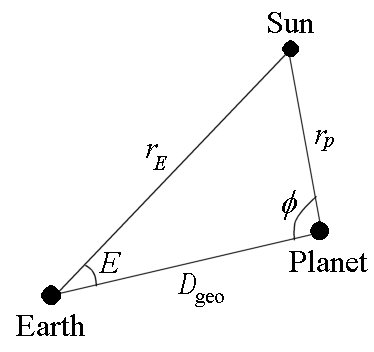
\includegraphics[width=6cm]{elongation_phaseAngle.jpg}
\end{center}
\caption{Elongation $E$ and phase angle $\phi$ of a planet.}
\label{fig:ElongPhaseAng}
\end{figure}

As shown in Figure~\ref{fig:ElongPhaseAng}, elongation $E$ of a planet is the angular 
distance between the Sun and planet as seen from Earth. Phase angle $\phi$ of a planet 
is the angular distance between the Sun and Earth as seen from the planet. It follows 
from the law of cosine that 
\beq
  \cos E = \frac{r_E^2 + D_{\rm geo}^2 - r_p^2}{2 r_E D_{\rm geo}} \ \ , \ \ 
  \cos \phi = \frac{r_p^2 + D_{\rm geo}^2 - r_E^2}{2 r_p D_{\rm geo}} ,
\label{eq:ElongPhaseAng}
\eeq
where $r_E$ is the heliocentric distance of the Earth, $r_p$ is the heliocentric 
distance of the planet, and $D_{\rm geo}$ is the geocentric distance of the 
planet. This formula ignores the finite speed of light. 
In principle, ray tracing is needed if high precision 
is required. More accurate formulae are 
\beq
  \cos E(t) = -\frac{\ve{r}_E(t) \cdot \ve{X}_p(t)}{|\ve{r}_E(t)| |\ve{X_p}(t)|} \ \ , \ \ 
  \cos \phi(t) = -\frac{[\ve{r_E}(t_r)-\ve{r_p}(t)] \cdot \ve{r_p}(t)}
{|\ve{r_E}(t_r)-\ve{r_p}(t)| |\ve{r_p}(t_r)|} ,
\eeq
where the retarded time $t_r$ satisfies the equation 
$t_r=t-|\ve{r_E}(t_r)-\ve{r_p}(t)|/c$ and 
we ignore the Sun's motion with repsect to the solar system barycenter, aberration 
of light and gravitational deflection of light.
The equation for the elongation is easy to calculate. It follows 
from 
\beqn
  \ve{r_E} &=& - r_E \left( \begin{array}{c} 
\cos \alpha_{\odot} \cos \delta_{\odot} \\ 
\sin \alpha_{\odot} \cos \delta_{\odot} \\ 
\sin \delta_{\odot} \end{array} \right) \\ \cr 
\ve{X_p} &=& |\ve{X_p}| \left( \begin{array}{c} 
\cos \alpha_p \cos \delta_p \\ \sin \alpha_p \cos \delta_p \\ \sin \delta_p 
\end{array} \right)
\eeqn
and the addition formula of the cosine function that 
\beq
  \cos E = \sin \delta_{\odot} \sin \delta_p + 
\cos \delta_{\odot} \cos \delta_p \cos (\alpha_{\odot} - \alpha_p) .
\label{eq:Elong}
\eeq
Accurate computation of $\phi$ is slightly more involved. 
However, elongation and phase angle are usually not
quantities of great interest and so they are not calculated to 
high precision. We simply use 
equation~(\ref{eq:ElongPhaseAng}) and light-time correction is not done 
carefully for the three distances. 

In the popup box for a planet, the elongation is displayed accurate to $0.1^\circ$ 
and the direction of the planet relative to the Sun is indicated by either W or E. 
E means the planet is to the east of 
the Sun and W means it is to the west of the Sun. To be more specific, E means 
$\lambda_p-\lambda_{\odot} > 0$ and W means $\lambda_p-\lambda_{\odot} <0$. 
Here $\lambda_p$ and $\lambda_{\odot}$ are the ecliptic longitude of the planet 
and the Sun, respectively. The difference $\lambda_p-\lambda_{\odot}$ is restricted 
to the range $[-\pi,\pi)$.

It can be shown (see e.g., Section~17.4 of 
\href{https://www.amazon.com/Spherical-Astronomy-Robin-M-Green/dp/0521317797}
{Green, {\it Spherical Astronomy}, Cambridge University Press 1985}) that the fraction 
of a spherical planet illuminated by the Sun is 
\beq
  F = \frac{1+\cos \phi}{2} .
\eeq
In the popup box for a planet, $F$ is displayed to two decimal places. All planets 
are modelled as spheres, although the deviation from a sphere is substantial for Jupiter 
and Saturn. The value of 
$F$ for Jupiter, Saturn, Uranus and Neptune is almost 1 at all times because of their 
large distances from the Sun. 

\subsubsection{Apparent Magnitude}

The apparent magnitude of a planet depends on its heliocentric distance $r_p$, 
geocentric distance $D_{\rm geo}$ and its phase angle $\phi$. The magnitude 
can be written as
\beq
  m = m_0 + 5\log_{10} \frac{r_p D_{\rm geo}}{{\rm AU}^2} + \Delta m(\phi) ,
\eeq
where $m_0$ is a constant and $\Delta m(\phi)$ is the variation of apparent 
magnitude as a function of $\phi$. The variation arises from the fraction of 
the planet illuminated and the property of diffuse reflection from the planet's 
surface/atmosphere. The function $\Delta m(\phi)$ is determined empirically and is 
listed in Table~10.6 of \expl and 
\href{http://aa.usno.navy.mil/publications/docs/exp_supp_errata.pdf}{errata}. 
The table is reproduced below with errors corrected. The phase angle $\phi$ is 
in degrees.

\begin{tabular}{ccc}
\hline
 Planet & $m_0$ & $\Delta m$ \\ 
\hline
 Mercury & -0.60 & $0.0498 \phi - 0.000488 \phi^2 + 3.02\times 10^{-6} \phi^3$ \\ 
 Venus & -4.47 & $0.0103\phi + 5.7\times 10^{-5} \phi^2 + 1.3\times 10^{-7} \phi^3$ 
for $2.2^\circ < \phi < 163.6^\circ$ \\ 
 Venus & 0.98 & $-0.0102\phi$ for $163.6^\circ < \phi < 170.2^\circ$ \\ 
Mars & -1.52 & $0.016\phi$ \\ 
Jupiter & -9.40 & $0.005\phi$ \\ 
Saturn & -8.88 & $0.044\phi - 2.6 |\sin e| + 1.25\sin^2 e$ \\ 
Uranus & -7.19 & $0.002\phi$ \\ 
Neptune & -6.87 & 0 \\
\hline
\end{tabular}

Note that $\Delta m$ is undefined for Venus when $0^\circ < \phi < 2.2^\circ$ and 
when $170.2^\circ < \phi < 180^\circ$. In the popup box, the expression for 
$2.2^\circ < \phi < 163.6^\circ$ is used when $0^\circ < \phi < 2.2^\circ$ 
and the expression for $163.6^\circ < \phi < 170.2^\circ$ is used when 
$170.2^\circ < \phi < 180^\circ$.

Saturn's magnitude calculation is more complicated because its rings have 
significant contribution to Saturn's brightness. As a result, the terms 
$- 2.6 |\sin e| + 1.25\sin^2 e$ appear in the formula for Saturn's magnitude. 
Here $e$ is the Saturnocentric sub-Earth latitude, which determines the orientation 
of Saturn's rings seen from Earth. The value of $e$ is computed as follows.
First compute the J2000.0 Ra and Dec of Saturn's north pole according to 
\beq
  \alpha_0 = 40.^{\circ}589 - 0.^{\circ}036 T \ \ , \ \ 
  \delta_0 = 83.^{\circ}537 - 0.^{\circ}004 T ,
\eeq
where $T$ is the TT Julian century from J2000.0. Next compute the 
unit vector $\ve{e_3}$ pointing in the direction of Saturn's rotation axis:
\beq
\ve{e_3} = \left( \begin{array}{c} 
\cos \delta_0 \cos \alpha_0 \\ \cos \delta_0 \sin \alpha_0 \\ \sin \delta_0 
\end{array} \right) 
\label{eq:SaturnE3}
\eeq
Finally, the value of $\sin e$ is given by 
\beq
  \sin e = \frac{\ve{X_S}\cdot \ve{e_3}}{|\ve{X_S}|} ,
\eeq
where $\ve{X_S}$ is Saturn's geocentric position.

\section{Moon}

\subsection{Lunar Ephemeris}

Position of the Moon is calculated based on the ELP/MPP02 series. A JavaScript 
code is created based on the source code provided by the authors on 
\href{ftp://cyrano-se.obspm.fr/pub/2_lunar_solutions/2_elpmpp02/}{this ftp site}. 
The JavaScript code has been tested by comparing the results with those of the 
FORTRAN code on the ftp site. We find agreement to within 12 to 13 significant figures. 
The deviation is most likely caused by the accumulated roundoff error. 

\href{http://adsabs.harvard.edu/abs/2003A%26A...404..735C}{ELP/MPP02} \
is a semi-analytic solution for the lunar motion. There are 
parameters in the model that are fitted to either the lunar 
laser ranging (LLR) data or fitted to JPL's DE405/DE406 ephemerides. 
Parameters fitted to DE405/DE406 are used on our webpages. The deviation between 
the positions in ELP/MPP02 and DE405/406 is less than $3.5''$ in ecliptic longitude 
and $0.8''$ in ecliptic latitude over the time span from 3000~BC to 3000~AD. 

The full ELP/MPP02 series can be written in the form 
\beqn
  V(T) &=& W(T) + \sum_{i=0}^3 T^i \sum_j A^{(V)}_{ij} \sin\left[ \phi^{(V)}_{ij}(T)\right] \\ 
  U(T) &=& \sum_{i=0}^3 T^i \sum_j A^{(U)}_{ij} \sin\left[ \phi^{(U)}_{ij}(T)\right] \\ 
  r(T) &=& r_0 + \sum_{i=0}^3 T^i \sum_j A^{(r)}_{ij} \sin\left[ \phi^{(r)}_{ij}(T)\right] ,
\label{eq:Dmoon}
\eeqn
where $V$, $U$, and $r$ are the ecliptic longitude, ecliptic latitude, and geocentric 
distance of the Moon, respectively, $T$ is the TT Julian century from J2000.0, 
$W$ is the mean longitude of the Moon, $r_0$ is a constant. For the terms in the 
sum, $A^{(U)}_{ij}$, $A^{(V)}_{ij}$, $A^{(r)}_{ij}$ are constants. The phase 
angles $\phi^{(U)}_{ij}$, $\phi^{(V)}_{ij}$, $\phi^{(r)}_{ij}$ are linear functions 
of 13 angles $a_k$ $(k=1,2,\cdots, 13)$ related to the mean positions and orbital 
parameters of the Moon and solar system planets. The functions $W(T)$ and $a_k(T)$ 
are expressed as polynomial functions of $T$ up to and including $T^4$. 

The full series involves about 36,000 terms. Since high accuracy is not 
needed for our use, we truncate the series by the following procedure:\footnote{I 
have created \href{https://github.com/ytliu0/ElpMpp02}{this GitHub repository} to 
provide C++ subroutines to implement the ELP/MPP02 series, construct 
truncated series, and generate JavaScript code to calculate the truncated series.}

\begin{itemize}
\item Choose four parameters $A^{(U)}_{\rm th}$, $A^{(V)}_{\rm th}$, 
$A^{(r)}_{\rm th}$ and $\tau$. 

\item Drop the terms in the series with $A^{(U)}_{ij} < A^{(U)}_{\rm th} /\tau^i$, 
$A^{(V)}_{ij} < A^{(V)}_{\rm th} /\tau^i$, and 
$A^{(r)}_{ij} < A^{(r)}_{\rm th} /\tau^i$.
\end{itemize}

It is clear that the smaller the parameters $A^{(U)}_{\rm th}$, $A^{(V)}_{\rm th}$, 
and $A^{(r)}_{\rm th}$, the closer the truncated series is to the original series. 
The parameter $\tau$ has a unit of time and is chosen to be 50~Julian centuries, 
which is the time span covered by the ELP/MPP02 series. Two sets of truncated 
series are created using two set of parameters. We call the two sets of 
truncated series ELP/MPP02L and ELP/MPP02C.

ELP/MPP02L is a low-precision series, created using 
$A^{(U)}_{\rm th}=A^{(V)}_{\rm th}=30''$, $A^{(r)}_{\rm th}=100$~km, and $\tau = 50$~Julian centuries. It is used for plotting the Moon on our star charts. 
The resulting series consists of about 40 terms. 
The accuracy of ELP/MPP02L is estimated by comparing it with the full series. 
Specifically, 10,000 random values of $T$ are chosen between -50 and 50. Values of 
$U(T)$, $V(T)$, and $r(T)$ at these times are computed for both the ELP/MPP02L series and the 
full series. We find that the maximum differences between ELP/MPP02L and ELP/MPP02 
are $233''$ for $V$, $152''$ for $U$ and $352$~km for $r$. The root mean square 
of the differences are $47''$ for $V$, $33''$ for $U$ and $86$~km for $r$. This accuracy 
is sufficient for our plotting purpose.

ELP/MPP02C is created using $A^{(U)}_{\rm th}=A^{(V)}_{\rm th}=0.001''$, 
$A^{(r)}_{\rm th}=0.1$~km, and $\tau = 50$~Julian centuries. It is used in 
the calculation in the popup box. The resulting series consists of about 3750 terms. 
The accuracy of ELP/MPP02C is estimated in the same way as above. We find that 
the maximum differences between ELP/MPP02C and ELP/MPP02 over the time 
span $|T|<50$ are $0.1''$ for $V$, $0.08''$ for $U$ and $1.9$~km for $r$. 
The root mean square of the differences are $0.02''$ for $V$, $0.01''$ for 
$U$ and $0.4$~km for $r$. The error of this truncated series is lower than 
the error of the apparent position caused by our ignoring the effect of 
polar motion.

Once $U$, $V$ and $r$ are computed, rectangular components of the geocentric 
position of the Moon with respect to the mean ecliptic and equinox of J2000.0 
are obtained by taking into account precession and transformation from spherical 
to Cartesian coordinates. The procedure is described in the pdf document on the ftp site. 
Equatorial coordinates of J2000.0 mean equator and equinox are then computed 
by rotating the ecliptic coordinates by the angle $\epsilon_0=23^\circ 26' 21.406''$ 
(obliquity of the ecliptic at J2000.0) about the $x$-axis. 
The J2000.0 equatorial coordinates are basically the GCRS coordinates, 
apart from the tiny difference 
between these two systems caused by the 23-milliarcsecond offset, which we ignored. 
Light-time correction is implemented by first computing the geocentric 
distance $r(t)$ using equation~(\ref{eq:Dmoon}). Then the retarded geocentric 
position is calculated by $\ve{X}(t_r) = \ve{X}(t-r(t)/c)$. Light-time correction 
shifts the Moon's position by about $1''$. Hence we ignore the light-time 
correction when using the low-precision ELP/MPP02L series. 

\subsection{Plotting the Moon} 

GCRS position of the Moon is calculated using the low-precision ELP/MPP02L 
series. GCRS Ra and Dec are then calculated using $\alpha={\rm arg}(X+iY)$ 
and $\delta=\sin^{-1}(Z/r)$. The Moon can now be plotted 
on the GCRS charts: its canvas coordinates are given by 
equations~(\ref{eq:stereographicXg})--(\ref{eq:mollweide}).

For the local star charts, we need to compute the altitude $a$
and azimuth $A$ at the given location. First, the ``of date'' geocentric equatorial
coordinates are computed by applying the precession matrix on $\ve{X}$. 
Since the Moon is close to the Earth, we need to account for the geocentric 
parallax by computing its topocentric position using 
equations~(\ref{eq:topoX})--(\ref{eq:topoCS}). The ``of date'' topocentric Ra and Dec
is then calculated by $\alpha_{\rm topo} = {\rm arg}(X_{\rm topo}+iY_{\rm topo})$ and 
$\delta_{\rm topo}=\sin^{-1} (Z_{\rm topo}/D_{\rm topo})$, where 
$D_{\rm topo}=\sqrt{X_{\rm topo}^2 + Y_{\rm topo}^2 + Z_{\rm topo}^2}$ is 
the topocentric distance of the Moon.
The hour angle is given by $H=t_s-\alpha_{\rm topo}$, where $t_s$ is the local
sidereal time (LMST). Next $a$ and $A$ are computed using
equations~(\ref{eq:aAFromHdel1})--(\ref{eq:aAFromHdel3}). Then the altitude
is adjusted by the atmospheric refraction according to equation~(\ref{eq:atmRefraction}).
The Moon can now be plotted on a local star chart: its canvas coordinates are
given by equation~(\ref{eq:stereographicHor}).

\subsection{Popup Box}

In the popup box, the Moon's position is calculated using the higher precision 
ELP/MPP02C and with light-time correction. Geocentric position, topocentric 
position, altitude and azimuth are computed in the same way as described above when 
the time is outside the interval 3000~BC--3000~AD. For times within the interval 
3000~BC--3000~AD, the J2000.0 positions
include only the light-time correction and geocentric parallax (for topocentric
position). The apparent ``of date'' position, as well as altitude and azimuth,
includes light-time correction,
precession, nutation and aberration of light. The calculations are the same
as those described in Section~\ref{sec:starsPopup}.

\begin{figure}[h]
\begin{center}
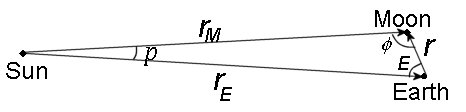
\includegraphics[width=10cm]{sunEarthMoon.jpg}
\end{center}
\caption{Geometry of the Sun, Moon and Earth.}
\label{fig:SunMoonEarth}
\end{figure}

Elongation $E$ and phase angle $\phi$ can be calculated using equations similar to 
equation~(\ref{eq:ElongPhaseAng}). However, it is easier to use 
equation~(\ref{eq:Elong}) to calculate $E$. For $\phi$, we need to 
compute the Moon's heliocentric position $\ve{r_M}$. As shown in 
Figure~\ref{fig:SunMoonEarth}, $\ve{r_M}=\ve{r_E}+\ve{r}$, where 
$\ve{r_E}$ is the heliocentric 
position of the Earth and $\ve{r}$ is the geocentric position of the Moon. 
It follows that 
\beq
  r_M^2 = |\ve{r_E}+\ve{r}|^2 = r_E^2 + 2\ve{r}\cdot \ve{r_E} + r^2 = 
r_E^2 - 2 r r_E \cos E+r^2 = r_E^2(1-2\sigma \cos E + \sigma^2) ,
\eeq
where $\sigma=r/r_E$ and we have used the fact that 
$\ve{r}\cdot \ve{r_E}=-r r_E \cos E$. The phase angle can be written as 
\beq
  \cos \phi = \frac{r_M^2+r^2-r_E^2}{2rr_M} = \frac{\sigma - \cos E}
{\sqrt{1-2\sigma\cos E + \sigma^2}} .
\label{eq:ElongMoon}
\eeq
Since $r \approx 3.8\times 10^{5}$~km and $r_E\approx 1.5\times 10^8$~km, 
$\sigma \approx 2.5\times 10^{-3} \ll 1$. Hence $\cos \phi \approx -\cos E$ or 
$\phi \approx \pi - E$. This approximate relation between $E$ and $\phi$ can 
be understood geometrically. As seen in Figure~\ref{fig:SunMoonEarth}, when 
$r \ll r_M$ and $r \ll r_E$, the line joining the Moon and the Sun and the 
line joining the Earth and the Sun are nearly parallel. It follows from the 
Euclidean geometry that $\phi + E = \pi$ if the two lines were parallel. Since 
the two lines are nearly parallel, the relation is approximate.
The difference between $\phi$ and $\pi - E$ is of 
order $\sigma \approx 2.5\times 10^{-3}$ radians or $0.15^\circ$. This accuracy 
is in fact adequate for our purpose since $\phi$ is only used to compute the 
fraction of the Moon illuminated $F=(1+\cos \phi)/2$. An error of $2.5\times 10^{-3}$ 
in $\phi$ results in the error in $F$ of order $10^{-3}$. We only display 
$F$ to 2 decimal places in the popup box 
and so this error is an order of magnitude smaller. In our code, however, 
we improve the approximation $\phi=\pi-E$ by replacing $r$ by its 
average value $384400$~km and replacing 
$r_E$ by its average value 1~AU$=149597870$~km. Hence $\sigma=r/r_E$ is replaced 
by $\sigma=2.57\times 10^{-3}$ and equation~(\ref{eq:ElongMoon}) can still 
be calculated easily. This correction pushes the error in $\cos \phi$ down to order 
$10^{-4}$.

\section{Rise, Set, Upper Transit and Twilight}

The rise, set, and upper transit times of celestial objects, as well as the beginning and 
ending of twilight, are computed in the popup box, and on the rise/set page when  
the Rise and Set Times button on the local star chart page is clicked. This section describes 
the method and algorithm used to do the calculation.

The rise and set times of a celestial object are defined as the times 
when the upper limb of the object touches the horizon.
Since the horizon depends on the observer's 
location, the rise and set times are different for different observers. 
The rise and set times are the times when the apparent {\em topocentric 
altitude} of the upper limb of the object is 0. 
The {\em geocentric altitude} of the {\em object's center} at the rise and set 
times is 
\beq
  a_{rs} = p - \Delta a - s , 
\eeq
where $p$ is the geocentric parallax, $\Delta a$ is the correction of the 
altitude due to atmospheric refraction and $s$ is the angular radius of the 
object. The atmospheric refraction term $\Delta a$ varies depending on the 
local conditions. For the Sun and Moon, $p$ and $s$ also vary slightly. Since 
the rise and set times are usually calculated to an accuracy of a couple of minutes, 
average values of $\Delta a$, $p$ and $s$ are used. The term $\Delta a$ is usually set 
to $34'$. For the Sun, $p \approx 8.8''$, $s\approx 16'$ and so $a_{rs}=50'$ for 
sunrise and sunset. For the Moon, $p\approx 57'$, $s\approx 15'$ and so $a_{rs}=8'$. 
For planets and stars, $p \ll \Delta a$ and $s \ll \Delta a$, and so we simply 
set $a_{rs}=-34'$. 

Twilight is usually divided into three phases. The beginning and ending 
of the {\em civil twilight} are the times when the Sun's center is $6^\circ$ below 
the horizon. When the civil twilight ends, the sky is dark enough for the 
brightest stars to be visible. The beginning and ending of the {\em nautical 
twilight} are the times when the Sun's center is $12^\circ$ below the horizon. When the 
nautical twilight ends, the sky is so dark that the horizon is no longer visible. 
The beginning and ending of the {\em astronomical twilight} are the times when 
the Sun's center is $18^\circ$ below the horizon. They mark the beginning and ending 
of the night time. When the astronomical twilight ends, the faintest stars 
are visible (in regions with clear sky and no light pollution). Thus, we have $a_{rs}=-6^\circ$ 
for civil twilight, $a_{rs}=-12^\circ$ for nautical twilight and 
$a_{rs}=-18^\circ$ for astronomical twilight.

Transits are defined as the times when the object crosses the meridian, which are 
the times when the hour angle of the object is 0 or $\pi$. The $H=0$ transit 
is called the {\em upper transit} and the $H=\pi$ transit is called the 
{\em lower transit}. 

Since the rise, set, and upper transit time calculation does not require high 
precision. Low-precision formulae for the positions of the Sun, Moon and planets 
are used. In addition, nutation, polar motion, aberration of light, and gravitational 
deflection of light by the Sun are ignored.

\subsection{Stars}

The rise and set times of stars can be computed relatively easily since their 
``of date'' right ascension and declination do not change much during the 
course of a day.

It follows from equation~(\ref{eq:aAFromHdel3}) that 
\beq
  \cos H = \frac{\sin a - \sin \delta \sin \phi}{\cos \delta \cos \phi} .
\label{eq:cosH}
\eeq
Here $\delta$ is the ``of date'' declination of the star. 
Since $-1 \leq \cos H \leq 1$, we have 
\beq
  -1 \leq \frac{\sin a - \sin \delta \sin \phi}{\cos \delta \cos \phi} \leq 1
\eeq
or 
\beq
  -\cos \delta \cos \phi + \sin \delta \sin \phi \leq \sin a \leq 
  \cos \delta \cos \phi + \sin \delta \sin \phi .
\eeq
It follows from the addition formula of the cosine function that 
\beq
  -\cos (\delta + \phi)  \leq \sin a \leq \cos (\delta - \phi) 
\eeq
which can be written as 
\beq
  \sin (|\delta + \phi| - 90^\circ) \leq \sin a \leq \sin (90^\circ - |\delta -\phi|) .
\eeq
Since $|\delta|\leq 90^\circ$ and $|\phi| \leq 90^\circ$, we have 
$|\delta + \phi| - 90^\circ \in [-90^\circ, 90^\circ]$ and 
$90^\circ - |\delta -\phi| \in [-90^\circ, 90^\circ]$. By definition, the 
amplitude $a \in [-90^\circ, 90^\circ]$. Since sine is an increasing function 
in $[-90^\circ, 90^\circ]$, we have 
\beq
  |\delta + \phi| - 90^\circ \leq a \leq 90^\circ - |\delta -\phi| .
\eeq
The minimum and maximum geocentric altitude are 
\beq
  a_{\rm min} = |\delta + \phi| - 90^\circ \ \ , \ \ 
  a_{\rm max} = 90^\circ - |\delta -\phi| .
\eeq
The maximum altitude occurs when the hour angle $H=0^\circ$, which is the upper transit.
The minimum altitude occurs when $H=180^\circ$, which is the lower transit.

For a given latitude $\phi$, there are stars with $a_{\rm min} > a_{rs}$. 
These stars are always above the horizon. They are called the {\em circumpolar stars}. 
A star is circumpolar if its declination satisfies the condition 
$\delta > 89^\circ 26' - \phi$ or $\delta < -(89^\circ 26' + \phi)$. 
Since $|\delta|\leq 90^\circ$, only the first inequality is relevant for 
northern hemisphere observers with $\phi > 34'$. Only the second inequality 
is relevant for southern hemisphere observers with $\phi < -34'$. Both inequalities 
are relevant only for observers very close to the equator with $|\phi|<34'$.

There are also stars with $a_{\rm max} < a_{rs}$. These stars are always 
below the horizon. They are always invisible at the location. A star is always 
invisible if its declination satisfies the condition $\delta < -(90^\circ 34' - \phi)$ 
or $\delta > 90^\circ 34' + \phi$. Only the first inequality is relevant 
for observers with $\phi > 34'$. Only the second inequality 
is relevant for observers with $\phi < -34'$. For observers
with $|\phi| \leq 34'$, there are no stars that are always invisible.

Thus the rise and set times are for stars that are not circumpolar and not always 
invisible. For these stars, the hour angle at the rise and set times are given by 
equation~(\ref{eq:cosH}) with $a=a_{rs}$: 
\beq
  H_{\pm} = \pm \cos^{-1} \frac{\sin a_{rs} - \sin \delta \sin \phi}{\cos \delta \cos \phi} ,
\eeq
When $H>0$, the star is on the west side of the meridian. When $H<0$, the star is 
on the east side of the meridian. Thus, the $+$ sign is for the set time and $-$ sign is 
for the rise time. The sidereal time at the rise and set times are given by 
\beq
  t_{s\pm}= H_{\pm} + \alpha ,
\eeq
where $\alpha$ is the ``of date'' right ascension of the star. Over the course 
of a day, the sidereal time advances at a rate 1.00273781191135448 faster than 
the clock time based on UTC, as indicated by equation~(\ref{eq:GMST}) (terms involving 
$T$ are practically constant over the course of a day). To calculate the 
rise and set times at a given time zone, we first calculate the sidereal time $t_{s0}$ 
at the midnight of the given time zone by 
\beq
  t_{s0}={\rm LMST}(D_{Um},T(D_{Um})) = {\rm GMST}(D_{Um},T(D_{Um})) + \lambda ,
\eeq
where $\lambda$ is the location's longitude, 
$D_{Um}= {\rm Julian~UT1~date~at~midnight~local~time}-2451545.0$, and $T(D_{Um})$ 
is the TT Julian century from J2000.0 at $D_{Um}$. In other words, 
\beq
  T(D_{Um}) = \frac{D_{Um}}{36525} + \Delta T(D_{Um}) ,
\eeq
where $\Delta T$ is the difference between TT and UT1 described in Section~\ref{sec:DeltaT}. 
The Greenwich sidereal time GMST is calculated using equation~(\ref{eq:GMST}) and 
$\Delta T$ is calculated using the fitting formula by 
\href{https://eclipse.gsfc.nasa.gov/SEcat5/deltatpoly.html}{Espenak and Meeus}. 
The sidereal time $t_s$ at any later time of the date is given by 
$t_s=t_{s0}+1.00273781191135448 h'$, where $h'=24(D_U-D_{Um})$ is the number of hours 
past the local midnight. The local times at which the setting and rising of the star 
occur on a given date are 
\beq
  h'_{\pm} = \frac{(H_{\pm} + \alpha - t_{s0})~{\rm mod}~24^{\rm h}}{1.00273781191135448} .
\label{eq:riseSetStars}
\eeq
Upper transit time is the time when the hour angle $H=0$. Hence 
\beq
  h'_{\rm upper~transit} = \frac{(\alpha - t_{s0})~{\rm mod}~24^{\rm h}}{1.00273781191135448} .
\label{eq:upperTransitStars}
\eeq
Note that equations~(\ref{eq:riseSetStars}) and (\ref{eq:upperTransitStars}) imply 
that $h'$ can never be greater than $24/1.00273781191135448$. This is because 
one sidereal day is $1/1.00273781191135448~{\rm days}=23^{\rm h} 56^{\rm m} 
4^{\rm s}$ and is smaller than 24 hours. Thus, if the rise/set/upper transit 
time occurs bewteen $0^{\rm h}$ and $0^{\rm h} 03^{\rm m} 56^{\rm s}$, there will 
be another rise/set/upper transit occurring on the same day with 
$h' > 24/1.00273781191135448$. This occurs only once every year for each case 
and we ignore them.

\subsection{Sun, Moon and Planets}

The equations for the rise, set, upper transit times of the Sun, Moon and planets, 
as well as the beginning and ending of twilight, are still given by 
equations~(\ref{eq:riseSetStars}) and (\ref{eq:upperTransitStars}). 
The only difference is that the right ascension and declination for
the Sun, Moon and planets change more rapidly over the course of a day.
The two equations should be written more clearly as follows.
\beqn
  h'_{\pm} &=& \frac{(H_{\pm}(\delta(h'_{\pm})) + \alpha(h'_{\pm}) - t_{s0})
~{\rm mod}~24^{\rm h}}{1.00273781191135448} 
\label{eq:riseSetPlanets} \\ \cr 
  h'_{\rm upper~transit} &=& \frac{(\alpha(h'_{\rm upper~transit}) - t_{s0})
~{\rm mod}~24^{\rm h}}{1.00273781191135448} 
\label{eq:upperTransitPlanets}
\eeqn
These equations explicitly indicate that the rise/set/upper transit time 
depends on the values of $\alpha$ and $\delta$ at the rise/set/upper transit time. 
Since $\alpha$ and $\delta$ can no longer be considered as constants over the 
course of a day, we have the unknown rise/set/upper transit time appearing 
on both sides of the equations. The equations may be solved iteratively. For the 
Sun and planets, $\alpha$ and $\delta$ change slowly over the course of a day. 
Treating them as constants will not cause an error of more than a few minutes, 
which is sufficient. However, the Moon moves rapidly over the course of a day 
and treating $\alpha$ and $\delta$ as constants will cause a large error.

There are two other complications. The time between two successive 
rise/set/upper transit times is one sidereal day for stars. This is not true 
for the Sun, Moon and planets. The most extreme case is the Moon, where the 
average time between two successive rise/set/upper transit times is 24 hours 
and 50 minutes. As a result, it is possible to have no rise/set/transit on 
a given day. Another complication is that at high latitudes, the rise and set 
times of the Sun, Moon and planets are sensitive to the change in declination 
when the object is close to being circumpolar or close to being invisible all day. 
These two complications make the iterative procedure difficult to implement. As 
a result, we use the algorithm described in Sections~3.7 and 3.8 of the book 
\href{https://www.springer.com/us/book/9783540672210#}{\it Astronomy on the 
Personal Computer} by O.~Montenbruck and T.~Pfleger, 4th edition, Springer 2000 
(corrected fourth printing 2009) to calculate the rise, set and transit times. 
The algorithm is based on quadratic interpolation. 

The idea is to first calculate the hour angle $H(h')$ and altitude $a(h')$ at local times 
$0^{\rm h}$, $1^{\rm h}$, ..., $24^{\rm h}$, i.e.\ at 
$h'=0, 1, ..., 24$. Divide the day into 12 intervals: 
$[0^{\rm h}, 2^{\rm h})$, $[2^{\rm h}, 4^{\rm h})$, ..., $[22^{\rm h}, 24^{\rm h})$. 
Next values of $H(h')$ and $a(h')$ in each of the 12 intervals are approximated by 
a quadratic interpolation. Therefore, there are approximate analytic formulae for $H(h')$ and 
$a(h')$ throughout the day and the rise, set, 
and upper transit times are then solved by the equations $a(h')=a_{rs}$ and $H(h')=0$ 
using analytic expressions. 

The procedure for the rise, set, beginning and ending of twilight works as follows. 
For $h'$ in a particular time interval, define 
\beq
  x = h'-h'_0 \ \ \ , \ \ \ y = \sin [a(h')] - \sin a_{rs} ,
\eeq
where $h'_0$ is the mid-point of the time interval. Thus we have $x\in [-1,1)$ 
and $y=0$ at the rise and set times. 
Next, fit a quadratic curve $y(x)=c_2 x^2+c_1x+c_0$ in the interval 
based on the three values of $y$ at $x=-1$, 0 and 1: 
\beq
  y_- = y(-1)=c_2-c_1+c_0 \ \ , \ \ y_0=y(0)=c_0 \ \ , \ \ y_+=y(1)=c_2+c_1+c_0 .
\eeq
Values of $c_0$, $c_1$, and $c_2$ are easily solved to give 
\beq
  c_2 = (y_+ + y_0)/2 - y_0 \ \ , \ \ c_1 = (y_+ - y_-)/2  \ \ , \ \  c_0=y_0 .
\eeq
The quadratic equation $y(x)=0$ has roots if $c_1^2-4c_0c_2 \geq 0$ and the 
roots are given by $x_{\pm}=(-c_1\pm \sqrt{c_1^2-4c_0c_2})/(2c_2)$.
The quadratic function $y(x)$ 
reaches an extremum at $x_m=-c_1/(2c_2)$. However, the function $y(x)$ only applies 
in the interval $x\in [-1,1)$. In general, there can be 0, 1 or 2 roots in the interval 
$[-1,1)$. Let's consider these three cases. 

{\em Case 1}: There is no root in the interval $[-1,1)$. No rising and setting 
occurs in this time interval. Move on to the next time interval. 

{\em Case 2}: There is one root, $x_1$, in the interval $[-1,1)$. Either rising or 
setting occurs in this time interval at $h'=h'_0+x_1$. It is rising if $y_-<0$ and 
$y_+>0$; it is setting if $y_->0$ and $y_+<0$. 

{\em Case 3}: There are two roots, $x_1$ and $x_2$, in the interval $[-1,1)$. Suppose 
$x_2>x_1$. Then rising and setting both occur in this time interval and the extremum 
$x_m=(x_1+x_2)/2$ is also inside this interval. If $y(x_m) > 0$, the object rises 
at $h'=h'_0+x_1$, reaches a maximum altitude at $h'=h'_0+x_m$ and sets at 
$h'=h'_0+x_2$. If $y(x_m)<0$. The objects sets at $h'=h'_0+x_1$, reaches 
a minimum altitude at $h'=h'_0+x_m$ and rises at $h'=h'_0+x_2$. 

By going through all the 12 intervals, the rise and set times can be found. 
For the upper transit time, the calculation is done in a similar way. We set 
$y = H(h')$ in this case. Care must be taken when calculating the roots of $y=0$. 
If $\alpha(h')$ and $\delta(h')$ are constants, $y$ will be a linear function of $x$ 
and so $c_2=0$. For the Sun and planets, $\alpha(h')$ and $\delta(h')$ 
are nearly constants and so $y(x)$ is close to being a linear function with $|c_2|\ll 1$. 
One of the roots is close to $-c_0/c_1$ and the other is close to $-c_1/c_2$. 
The root close to $-c_0/c_1$ can be calculated using the expression $x_1=-2c_0/D$ 
and the one close to $-c_1/c_2$ can be calculated using $x_2=-D/(2 c_2)$, where 
$D=c_1+\sqrt{c_1^2-4c_0c_2}$ if $c_1>0$ and $D=c_1-\sqrt{c_1^2-4c_0c_2}$ if $c_1<0$. 
Since $|c_2|\ll 1$, it is almost certain that the root close to $-c_1/c_2$ 
is outside the interval $[-1,1)$. Only the root close to $-c_1/c_2$ has a chance 
of being inside the interval $[-1,1)$. Normal celestial objects are not moving 
fast enough for there to be two upper transits occurring in a two-hour time interval 
and so we will never encounter Case~3. 

The algorithm described above has been tested on stars and the times computed 
match those calculated using equations~(\ref{eq:riseSetStars}) and 
(\ref{eq:upperTransitStars}). The difference is at most one minute.
As in the case of stars, on rare occasions there could be more than one 
rise/set/upper transit times for the Sun and planets on a day. The 
algorithm described above can find all of them, but only the earliest 
time is reported in the popup box and on the rise/set page.

\end{document}
